\documentclass[12pt]{report}

\usepackage[backend=biber,bibencoding=utf8,style=numeric]{biblatex}
\addbibresource{bibliografia.bib}

\usepackage[letterpaper, width=150mm,top=50mm,bottom=25mm]{geometry}
\setlength{\headsep}{0in}

\usepackage[utf8]{inputenc} %utf-8 encoding
\inputencoding{utf8}
\usepackage[spanish]{babel}
\usepackage{csquotes} %ensure proper quotations on babel and biblatex
\decimalpoint

\usepackage{tikz}
\usetikzlibrary{babel} % fix meaning of <>
\usetikzlibrary{arrows,backgrounds, fit, calc, bending, positioning}
\usepackage{pgfplots}
%\pgfplotsset{compat=1.12}

\usepackage{amssymb} %math symbols

\usepackage{multirow}

\usepackage{setspace}
\onehalfspacing
\setlength{\parindent}{4em}
\setlength{\parskip}{.5em}

\usepackage{array}
\usepackage{algorithm}
\usepackage{algpseudocode}

\usepackage{caption}
\usepackage{subcaption}

\usepackage{framed}

\usepackage{doc} %for bibtex logo
\usepackage{hologo} %for pdftex logo

%\usepackage{placeins}
%\usepackage{todonotes}

\usepackage{wrapfig}

\begin{document}

\begin{titlepage}
	\begin{center}                

		\begin{minipage}{4cm}
  	  
\includegraphics[width=4cm]{images/uach}
	  \end{minipage}
  	\hfill
	  \begin{minipage}{10cm}
	  	\centering
      UNIVERSIDAD AUTÓNOMA DE CHIHUAHUA \\[0.3\baselineskip]
  	  FACULTAD DE INGENIERÍA \\[0.3\baselineskip]
	    SECRETARÍA DE INVESTIGACIÓN Y POSGRADO \\[0.3\baselineskip]
    	MAESTRÍA EN INGENIERÍA EN COMPUTACIÓN
		\end{minipage}
			
		\vspace{1.5cm}

		\begin{doublespace}
			CÁLCULO DE GRADOS DE LIBERTAD EN MODELOS DE PROTEÍNAS Y ENTRAMADOS, ANÁLISIS DE DOS ALGORITMOS: PG Y VPG 
		\end{doublespace}

		\vspace{1cm}

    TESIS
        
		\vspace{1cm}

    (PARA OBTENER EL GRADO DE MAESTRO EN INGENIERÍA)
        
		\vspace{1cm}

		PRESENTA

		\vspace{1cm}
				     
		CARLOS MANUEL LICEA VÁZQUEZ
        
    \vfill
                
    CHIHUAHUA, CHIH. \hfill JUNIO 2016      
	\end{center}
\end{titlepage}

\newpage

\pagenumbering{gobble}

\begin{center}                
	\begin{minipage}{4cm}
  	
\includegraphics[width=4cm]{images/uach}
	 \end{minipage}
  \hfill
	\begin{minipage}{10cm}
	  \centering
    UNIVERSIDAD AUTÓNOMA DE CHIHUAHUA \\[0.3\baselineskip]
  	FACULTAD DE INGENIERÍA \\[0.3\baselineskip]
  	MAESTRÍA EN INGENIERÍA EN COMPUTACIÓN
	\end{minipage}
			
	\vspace{1cm}

	\begin{doublespace}
		CÁLCULO DE GRADOS DE LIBERTAD EN MODELOS DE PROTEÍNAS Y ENTRAMADOS, ANÁLISIS DE DOS ALGORITMOS: PG Y VPG 
	\end{doublespace}

	\vspace{.5cm}

  TESIS
        
	\vspace{.5cm}

  (PARA OBTENER EL GRADO DE MAESTRO EN INGENIERÍA)
        
	\vspace{.7cm}

	\begin{minipage}{0.5\linewidth}
		\begin{tabular}{c}
			APROBADO: \\
			\\[.7cm] \hline
			Luis Carlos González Gurrola, diretor \\
			\\[.7cm] \hline
			Fernando Martínez Reyes, sinodal \\
			\\[.7cm] \hline
			José Eduardo Acosta Cano de los Rios, sinodal
		\end{tabular}
	\end{minipage}
        
  \vfill

  CHIHUAHUA, CHIH. \hfill JUNIO 2016      
\end{center}

\newpage

\begin{center}
\large

\vspace*{6cm}
Copyright © \\[1cm]
por \\
Carlos Manuel Licea  Vázquez\\
2016
\vfill
\end{center}

\newpage
%oficio de la tesis
\newpage

\pagenumbering{roman}

% Paragraph customization

\chapter*{Resumen}
En la presente tesis se enumeran los diferentes métodos para cuantificar la rigidez de los cuerpos, específicamente rigidez local de entramados y proteínas. Se exponen algoritmos que la predicen según la descripción de los enlaces presentes y se implementan dos de ellos: los algoritmos PG y VPG. Se explican a profundidad los planteamientos, las rutinas y las asumciones que lo componen. Por último se caracterizan sus tiempos de corrida y se comparan los diferentes resultados obtenidos para diferentes entramados y características intrínsecas de redes.

\textbf{Palabras clave}: conteo de restricciones, conteo de grados de libertad, proteínas, tramados, análisis de rigidez, pebble game, virtual pebble game.

\chapter*{Abstract}
In this thesis different methods to quantify body rigidity are presented, specifically local rigidity for lattices and proteins. Some algorithms are presented that can predict rigidity solely with the description of the present edges, Two of them are implemented: the PG and VPG algorithms. Their assumptions, methods and, concepts that make them up. Later, running times are also characterized and compared for different lattices and intrinsic characteristics.

\textbf{Keywords}: restriction counting, degrees of freedom calculation, proteins, lattices, rigity analisis, pebble game, vitual pebble game.

\tableofcontents

\listoffigures

\listoftables

\newpage
 
\pagenumbering{arabic}

\chapter{Introducción}
Las proteínas son la maquinaria que hace funcionar a la célula en su totalidad. Las células expresan las proteínas según su código genético y estas a su vez llavan a cabo todas las funcionas biológicas. Respiración, reparación y reproducción, todas son llevadas a cabo según las proteínas creadas por la célula. Por esta razón es muy importante comprender cómo es que las proteínas interactúan con los diferentes mecanismos celulares y cómo llevan a cabo sus procesos.

Es bien sabido que la forma en que se plega una proteína es la que le confiere el uso biológico dentro de una célula. Éste plegado está definido por la rigidez de cada una de las áreas e influenciado por el medio en que ocurre el proceso. Dentro de los diferentes métodos que existen para inferir esta rigidez se encuentran el de conteo de restricciones.

Así, en el presente trabajo se presenta la reimplementación de los algoritmos de conteo de restricciones PG y VPG para análisis de rigidez de cuerpos en general y de proteínas específicamente. 

Además la reimplementación de los algoritmos se hará de una manera que se pueda reutilizar el código para que sirva de base para futuros trabajos, haciéndolo lo más eficiente y claro posible. Por último se comparan sus resultados y complejidad. Al final, éste trabajo permitiría agilizar los cálculos y solamente realizar aquellos para los que la tolerancia a la incertidumbre sea menor.

En el capítulo primero se introduce el trabajo en sí y además se plantean todo el marco de la tesis: el problema a atacar, los antecedentes, la justificación para emprenderlo, los objetivos y las hipótesis que sirve de ancla a la tesis.

En el capítulo segundo se introduce al lector al marco teórico y la teoría de grafos que respalda el uso de estas técnicas para el modelado de redes. Se explican todos los conceptos que se requieren para el completo entendimiento de la tesis. Se describen las diferentes técnicas para la comprensión de proteínas, tanto de laboratorio como analíticas y sus diferentes fortalezas y debilidades.

El capítulo tercero describe la metodología. Es decir, se detallan los algoritmos centrales a la tesis: el PG y el VPG y sus diferencias, además de presentar ejemplos correctos de su aplicación.

El capítulo cuarto presenta los experimentos y resultados obtenidos al implementar la metodología para la resolución de las hipótesis planteadas.

El capítulo quinto presenta discusiones sobre trabajos futuros.

El capítulo sexto cierra la tesis presentando las conclusiones finales de haber desarrollado el trabajo.

Los últimos dos capítulos presentan la bibliografía y figuras anexas así como los datos crudos y un vínculo al código desarrollado. 

\section{Antecedentes}
Muchas de las propiedades microscópicas de los cuerpos se pueden entender en función de la estructura microscópica\parencite{Jacobs97analgorithm} de los materiales. Trabajos previos en física computacional han demostrado la fiabilidad de modelar las estructuras de los compuestos mediante su estabilidad termodinámica. Específicamente en proteínas, hace décadas que se conoce que las regiones de flexibilidad de la proteína es lo que vincula su estructura con su función biológica\parencite{Gerstein1994}.
Aprovechando esto, múltiples técnicas han surgido para intentar predecir la flexibilidad en los diferentes radicales que conforman una proteína. Desde cristalografía con técnicas exploratorias en laboratorio hasta trabajos en biología computacional que permite la predicción únicamente mediante su composición (llamadas técnicas \emph{ab initio}).

Dentro de los métodos ab initio, es decir los que se dedican a inferir la flexibilidad únicamente mediante la descripción de los átomos en una proteína, se encuentra el Pebble Game (PB)\parencite{Jacobs97analgorithm}. Este representa los grados de libertad de las moléculas mediante guijarros que se consumen para mantener la estructura. Sin embargo, dada la naturaleza estadística de la mecánica cuántica y la termodinámica, específicamente que las interacciones de enlaces no covalentes se rompen y se vuelven a generar según el contexto térmico de la proteína, se requiere de múltiples ejecuciones para obtener un resultado que modele adecuadamente el comportamiento esperado.

Para paliar este costo computacional surge una aproximación de campo medio, es el conocido como Virtual Pebble Game (VPG)\parencite{Gonzalez2011} que reemplaza el costo de cada enlace por el costo esperado de cada enlace. Debido a esto puede ser que tenga un costo fraccionario, de ahí el nombre de guijarros virtuales.

Éste método, VPG, dada la flexibilidad de los guijarros virtuales, nos da resultados que aproximan muy adecuadamente a los obtenidos por PG sin necesidad de hacer los cálculos cientos de veces \parencite{Gonzalez2011}. Permitiendo además hacer simplificaciones a los cálculos aún más. 

Sin embargo, rápidamente se encontró que existen redes que por su caracterización hacen que la diferencia entre las predicciones de los algoritmos VPG y PG sean muy grandes y que, de hecho, la única forma de obtener la precisión del algoritmo PG es utilizándolo\parencite{Gonzalez2011}. El problema surge en que el algoritmo VPG es una aproximación y no un reemplazo al algoritmo PG y en ciertas circunstancias específicas la discrepancia entre uno y otro es muy considerable. Haciendo que  la única manera de obtener los resultados de PG es utilizando PG y no su aproximación.

Con la idea de mezclar los dos enfoques de PG --costo exaacto-- y VPG --costo medio--,  nace el algoritmo de VPG-x\parencite{Gonzalez2011} en el que un porcentaje x de los enlaces más significativos (los puentes de hidrógeno) se muestrearán mientras que para el resto se seguirá utilizando con la media. Esto nos permite reducir el margen de error en VPG y PG con un muestreo alrededor de 20 veces menor.
Para definir qué tanto se acerca las predicciones de ambos sistemas, se han intentado diferentes enfoques, en la propia tesis donde se presentó el algoritmo se introdujo un índice de heterogeneidad\parencite{Gonzalez2011}. Sin embargo no se logró una buena correlación. Después, haciendo uso de machine learning, una pequeña incursión se dio con programación genética\parencite{Chacon2014}, obteniendo resultados mixtos: por una parte se consiguió una correlación significativa con alrededor de 0.91 de explicación de la varianza pero el árbol obtenido es muy complejo y no se presta a obtener alguna relación apreciable analíticamente. Además de que se limitó a intentar predecir solamente la diferencia entre las predicciones de los grados de libertad. Dejándose de lado otras comparativas.

\section{Situación actual}
Desde la presentación del algoritmo VPG y sus variantes no ha habido ningún avance significativo con respecto a su caracterización. No se han presentado nuevas implementaciones, nuevos índices de heterogeneidad ni intentos para reducir la diferencia de predicción entre uno y otro, a pesar de que múltiples enfoques fueron aludidos en la propia tesis que convendría intentar. Por otra parte existen múltiples estrategias en la implementación de de mejorar aún más el desempeño con respecto a una implementación ingenua.

\section{Problema de investigación}
Actualmente el desconocimiento en muchos de los casos del comportamiento del algoritmo VPG-x no permite garantizar una adecuada aproximación minimizando la complejidad del algoritmo. El desconocimiento de opciones eficientes conlleva a una ralentización en la caracterización del comportamiento de las moléculas en general y a las proteínas en particular.  Esto causa un retraso en la investigación de nuevos compuestos y nuevas drogas para tratar los diferentes enfermedades o desórdenes metabólicos.

\subsection*{Preguntas de investigación}
Las preguntas de investigación se pueden plantear de la siguiente manera:
\begin{enumerate}
	\item ¿Se puede mejorar el tiempo de ejecución del algoritmo solamente mediante una aproximación?
	\item ¿Qué tanto intercambio entre aproximación y precisión se tiene cuando se aproxima el algoritmo PG mediante VPG?
	\item ¿Qué tanta diferencia en rapidez o uso de memoria hace una implementación que se aprovecha de las particularidades del problema sobre una que es ingenua y solamente considera un caso general?
\end{enumerate}

\section{Justificación}
La culminación de esta tesis permitirá contrastar las diferencias de comportamiento en tiempo y memoria entre PG y VPG. Además de encontrar un método rápido que nos permita obtener análisis ya sean de redes o de proteínas con la fidelidad adecuada sin gastar más tiempo del necesario.

Además, con este trabajo se obtendrá una mejor caracterización del algoritmo VPG que permita combinar las ventajas de los métodos de ensambles y el de campo medio.

\section{Delimitación}
El estudio se realizará únicamente utilizando como muestras las redes cristalinas que serán generados por un programa creado para este proceso. Se usará solamente el lenguaje de programación C++ y Python en los casos que se requiera un lenguaje adicional.

Se realizará en las instalaciones de la UACH con el apoyo del Doctor Luis Carlos González Gurrola y sin colaboraciones externas.

\section{Objetivo general}
Implementar y comprender los algoritmos de análisis de rigidez para entender los intercambios entre tiempo de ejecución, uso de memoria y exactitud del resultado final.

\section{Objetivos específicos}
\begin{enumerate}
  \item Implementar correctamente PG y VPG.
  \item Implementar los algoritmos eficientemente en memoria y tiempo.
  \item Comparar las implementaciones optimizadas contra implementaciones ingenuas.
\end{enumerate}

\section{Hipótesis}
\begin{enumerate}
	\item Se puede mejorar el tiempo de ejecución de un algoritmo solamente mediante la mejora de la representación del problema
	\item Las representaciones de campo medio son suficientes para aproximar en la mayoría de los casos las representaciones exactas
	\item El almacenar información calculada compleja en el modelo permite simplificar la resolución de problemas
\end{enumerate}

\chapter{Marco teórico} \label{marco}
\section{Modelado de redes}
Muchas de las propiedades macroscópicas de los cuerpos se pueden entender en función de la estructura microscópica\parencite{Jacobs1997}\parencite{Garboczi1985}\parencite{Guyon1990} de los materiales. Por ejemplo, la resistencia macroscópica depende del agregado de  resistencias microscópicas a la deformación. Usualmente lo que se estudia son corpúsculos, dependiendo de la escala a la que se haga el estudio pueden ser átomos, radicales u objetos, que se unen para formar un cuerpo con secciones rígidas o blandas. Al estudio y caracterización de la rigidez de estas secciones se le conoce como \emph{percolación de rigidez}.

Específicamente con respecto a las proteínas, hace décadas que se conoce que la flexibilidad de los diferentes segmentos de una proteína es la que vincula su estructura con su función biológica\parencite{Gerstein1994}.

Para estudiar la rigidez de los cuerpos existen dos métodos principales: experimentalmente y mediante modelado computacional. Para la primera se utilizan diferentes técnicas de cristalografía de rayos X o mediante resonancia magnética nuclear. Un ejemplo de uso de rayos X para inferir la forma de una molécula se presenta en la figura \ref{fig:dna}, la cual presenta la imagen que permitió deducir la forma en espiral del ADN obtenida mediante técnicas de cristalográfica desarrolladas por Rosalind Franklin y por trabajos de Aaron Klug.

\begin{figure}
\center
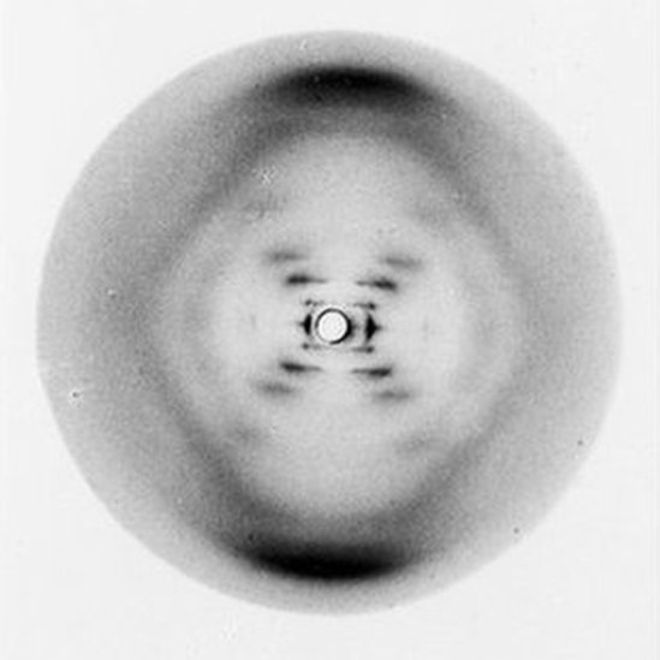
\includegraphics[width=70mm]{./images/adn}
\caption{Imágen obtenida mediante cristalografía de rayos X que demuestra la forma en espiral del ADN}
\label{fig:dna}
\end{figure}

El modelado computacional, por otra parte, presentan los siguientes tres paradigmas en general:\parencite{Ahmed2013}

\begin{enumerate}
\item Homología: en el que se identifican regiones similares a otras regiones cuyo comportamiento ya se conoce.
\item Reconocimiento de plegado: en la que se identifican las formas en que se pliegan las proteínas mediante su analogía con otros métodos.
\item \emph{Ab initio}: en la que se predice el comportamiento de la molécula solamente conociendo una descripción de los átomos que la componen. Mediante algoritmos especializados se encuentran las regiones rígidas y flexibles de las redes.
\end{enumerate}

El presente trabajo se centra únicamente en procesos del modelado \emph{Ab Initio}. Específicamente en los algoritmos PG y VPG. Estos predicen únicamente mediante una lista de los átomos que componen una red o proteína las partes rígidas y las partes flexibles mediante el uso de conteo de restricciones.

\section{Modelado mediante conteo de restricciones}
El modelado de estructuras mediante el conteo de restricciones consiste en representar el cuerpo a modelar mediante cuerpos más pequeños que se interconectan para formar un cuerpo más grande. Las conexiones mantienen a la estructura unida pero tienen un costo en grados de libertad para los nodos individuales. Es decir, para mantenerse unidas se pierde cierta cantidad de movimiento o rotación. La cantidad de grados que queda en cada nodo representa la rigidez o la flexibilidad del cuerpo.

La percolación es un problema complejo inherentemente no local, es decir, para determinar las propiedades de una región dada, se debe examinar detalles estructurales que se encuentran lejos de la zona. Estos detalles dificultaban significativamente la implementación de un algoritmo eficiente. Los primero intentos tenían tiempos de corrida que usualmente rondaban la complejidad $O(n^3)$ (una introducción sobre notación O-grande se presenta en la sección \ref{o-grande}). Sin embargo, el panorama cambió cuando se introdujo el algoritmo PG. Éste presenta una complejidad en el peor de los casos de $O(n^2)$ y que usualmente no excede $O(n^{1.15})$\parencite{Jacobs1997}.

Específicamente, PG representa la estructura mediante un grafo interconectado dirigido cuyos grados de libertad depende de la dimensionalidad del problema (6 para una red en tres dimensiones: movimientos y rotaciones en los tres ejes), estos son representados mediante \emph{pebbles} (guijarros) que son consumidos para mantener la estructura del material. Es decir, cada enlace que un átomo hace con otro le prohíbe moverse o rotar en un numero determinado de direcciones, dependiendo de la naturaleza de éste.

Aunque la complejidad computacional del algoritmo es mucho mejor que todo lo que se tenía hasta el momento, las constantes del polinomio se pueden considerar altas. Ya que, dada la naturaleza fluctuante de los enlaces atómicos hacen que el algoritmo deba de ejecutarse un número adecuado de veces para obtener un promedio que caracterice apropiadamente a la red.

Para paliar esto se presentó el algoritmo \emph{Virtual Pebble Game}(VPG)\parencite{Gonzalez2011} (Juego de Guijarros Virtuales) como una aproximación de campo medio. El VPG hace una simplificación importante: cambia los \emph{pebbles} enteros por \emph{pebbles} virtuales que pueden consumirse parcialmente para mantener la estructura, además cambia la manera en que el costo de cada enlace es asignado. Si antes el enlace se encontraba presente con una probabilidad $p$ de $costo$, ahora siempre se encuentra presente y el costo es simplemente $p*costo$.

El algoritmo, entonces, intercambia el muestreo por una aproximación de campo medio. Reduciendo la cantidad de ejecuciones a simplemente una debido a que se intercambian múltiples realizaciones a solamente una como se aprecia en la figura \ref{fig:realizaciones}. Los resultados obtenidos son muy buenos con todas las métricas, sin embargo existen ciertas configuraciones de red en donde las predicciones entre PG y VPG son muy dispares.

\tikzset{
    vertex/.style={circle, fill=black, minimum size = 7pt, inner sep=0pt},
    fluct/.style=dotted,
    array/.pic = {
        \foreach \i [count=\row] in {0,1}
            \foreach \j [count=\col] in {0,1,2,3}
                \node[vertex] (\row\col) at (\col,-\row) {};
        \draw (21)|-(13)|-(24)--(14);
        \draw (22)--(12);
    }
}

\begin{figure}
\centering

\setlength{\tabcolsep}{1cm}
\renewcommand{\arraystretch}{2}
\begin{tabular}{cr}
\multirow{4}{*} 	{
\begin{tikzpicture}[remember picture]
\pic (A) {array};
\path (A11) -- (A14) node[midway,above=3mm] {Una realización};
\draw[fluct] (A21)--(A23);
\end{tikzpicture}}
&
\begin{tikzpicture}[remember picture]
\pic (B) {array};
\path (B11) -- (B21) node[midway,left=3mm] (B_label) {Realización 1};
\draw[fluct] (B21)--(B22);
\node (R1) [left of = B_label, left=2mm] {};
\end{tikzpicture}
\\
&
\begin{tikzpicture}[remember picture]
\pic (C) {array};
\path (C11) -- (C21) node[midway,left=3mm] {Realización 2};
\draw[fluct] (C22)--(C23);
\end{tikzpicture}
\\
&
\begin{tikzpicture}[remember picture]
\pic (D) {array};
\path (D11) -- (D21) node[midway,left=3mm] {Realización 3};
\draw[fluct] (D21)--(D23);
\end{tikzpicture}
\\
&
\begin{tikzpicture}[remember picture]
\pic (E) {array};
\path (E11) -- (E21) node[midway,left=3mm] (E_label) {Realización 4};
\node (R4) [left of = E_label, left=2mm] {};
\end{tikzpicture}
\end{tabular}

\tikz[remember picture, overlay] \draw[thick, dotted,->] (A14) + (3mm,2mm) -- (R1);
\tikz[remember picture, overlay] \draw[thick, dotted,->] (A24) + (3mm,-2mm) -- (R4);

\caption{Diferencia de realizaciones entre VPG (izquierda) y PG (derecha).}
\label{fig:realizaciones}
\end{figure}

Para intentar solucionar el problema se introdujo VPG-x que vuelve a muestrear cierta porción de los enlaces. Aunque se reduce la ganancia en tiempo computacional, aún así los resultados no llegan a ser iguales al PG en ciertas condiciones.

Para aplicar los algoritmos se necesita tener la descripción de una red y una o múltiples realizaciones sea el caso del algoritmo que se desee aplicar.

\section{Descripciones de red y realizaciones} \label{descripciones-realizaciones}
Para la creación de la \emph{descripción} de una red es simple: se debe decidir en esencia para cada uno de los enlaces presentes si es que este se considera fijo --siempre presente-- o fluctuante y el costo que incurre cada nodo en mantener cada enlace.

La forma esto se determina varía según la naturaleza de la red. Si la red se crea artificialmente, el costo se puede decidir arbitrariamente y los enlaces se pueden crear al azar decidiendo qué porcentaje de enlaces se quieren fijos con una variable $q_fix$ (a veces nombrado \emph{background}) y qué porcentaje fluctuantes con una variable $q_fluct$; obviamente esto nos deja que existe un porcentaje de enlaces que no están presentes $q_{miss} = 1-q_{fix}-q_{fluct}$.

Mientras que si lo que se quiere resolver es una proteína o compuesto físico, el tipo de enlace químico determina el tipo de enlace en la red y su costo.

Dada la naturaleza probabilística de los enlaces fluctuantes es necesario crear \emph{realizaciones}. Aunque la creación de una red es idéntica para los dos algoritmos, las realizaciones varían fundamentalmente entre PG y VPG. En PG se usan para establecer para cada enlace fluctuante si se encuentra presente o no. Para ello se debe decidir con qué probabilidad es que estos estén presentes en la red eligiendo un hiperparámetro $p$ tal que $0\leq p \leq 1$ que representa la fracción de los enlaces fluctuantes que están presentes en la red o, análogamente, el porcentaje de veces que cada enlace está presente en las múltiples realizaciones. En VPG mientras tanto se aproxima el comportamiento anterior asumiendo que los enlaces fluctuantes siempre están presentes pero cambiando su costo por $p*cost$.

Se puede apreciar que $p$ abstrae todo el ambiente en el que la red se encuentra. Todos los factores que permitan que haya más enlaces presentes o que por el contrario prevenga que los enlaces fluctuantes se encuentren presentes. Para una proteína puede representar la cantidad de energía que hay en el ambiente.

Según la descripción de una red dada en la figura \ref{fig:descripcion-red}, $p=0.5$ y $cost=5.0$ se puede crear las posibles instancias para PG que se muestra en la figura \ref{fig:instancias-pg} y para VPG en la figura \ref{fig:instancias-vpg}.

\begin{figure}
\centering
\begin{tikzpicture}[align=center,node distance=2cm]
\tikzstyle{vertex}=[circle,draw=black]
\tikzstyle{fixed}=[->,semithick]
\tikzstyle{fluct}=[->,semithick, dotted]

\node[vertex] (v0) {$v_0$};
\node[vertex] (v1) [right of = v0] {$v_1$};
\node[vertex] (v2) [below of = v0] {$v_2$};
\node[vertex] (v3) [right of = v2] {$v_3$};

\path[every node] 
  (v0) edge [fixed] node[auto] {$e_1$} (v1)
  (v0) edge [fluct] node[auto] {$e_0$} (v2)
  (v1) edge [fixed] node[auto] {$e_2$} (v3)
  (v2) edge [fixed] node[auto] {$e_5$} (v3);
\end{tikzpicture}
\caption{Descripción de una red. Los enlaces punteados son fluctuantes y los sólidos fijos.}
\label{fig:descripcion-red}
\end{figure}

\begin{figure}
\centering
\begin{tikzpicture}[align=center,node distance=2cm]
\tikzstyle{vertex}=[circle,draw=black]
\tikzstyle{fixed}=[->,semithick]
\tikzstyle{fluct}=[->,semithick, dotted]

\node[vertex] (v0) {$v_0$};
\node[vertex] (v1) [right of = v0] {$v_1$};
\node[vertex] (v2) [below of = v0] {$v_2$};
\node[vertex] (v3) [right of = v2] {$v_3$};

\path[every node] 
  (v0) edge [fixed] node[auto, label={[font=\small]below:$5.0$}] {$e_1$} (v1)
  (v0) edge [fluct] node[auto, label={[font=\small]left:$5.0$}] {$e_0$} (v2)
  (v1) edge [fixed] node[auto, label={[font=\small]left:$5.0$}] {$e_2$} (v3)
  (v2) edge [fixed] node[auto, label={[font=\small]below:$5.0$}] {$e_5$} (v3);
\end{tikzpicture}
\qquad
\begin{tikzpicture}[align=center,node distance=2cm]
\tikzstyle{vertex}=[circle,draw=black]
\tikzstyle{fixed}=[->,semithick]
\tikzstyle{fluct}=[->,semithick, dotted]

\node[vertex] (v0) {$v_0$};
\node[vertex] (v1) [right of = v0] {$v_1$};
\node[vertex] (v2) [below of = v0] {$v_2$};
\node[vertex] (v3) [right of = v2] {$v_3$};

\path[every node] 
  (v0) edge [fixed] node[auto, label={[font=\small]below:$5.0$}] {$e_1$} (v1)
  (v1) edge [fixed] node[auto, label={[font=\small]left:$5.0$}] {$e_2$} (v3)
  (v2) edge [fixed] node[auto, label={[font=\small]below:$5.0$}] {$e_5$} (v3);
\end{tikzpicture}
\caption{Diferentes instancias para PG}
\label{fig:instancias-pg}
\end{figure}

\begin{figure}
\centering
\begin{tikzpicture}[align=center,node distance=2cm]
\tikzstyle{vertex}=[circle,draw=black]
\tikzstyle{fixed}=[->,semithick]
\tikzstyle{fluct}=[->,semithick, dotted]

\node[vertex] (v0) {$v_0$};
\node[vertex] (v1) [right of = v0] {$v_1$};
\node[vertex] (v2) [below of = v0] {$v_2$};
\node[vertex] (v3) [right of = v2] {$v_3$};

\path[every node] 
  (v0) edge [fixed] node[auto, label={[font=\small]below:$5.0$}] {$e_1$} (v1)
  (v0) edge [fluct] node[auto, label={[font=\small]left:$2.5$}] {$e_0$} (v2)
  (v1) edge [fixed] node[auto, label={[font=\small]left:$5.0$}] {$e_2$} (v3)
  (v2) edge [fixed] node[auto, label={[font=\small]below:$5.0$}] {$e_5$} (v3);
\end{tikzpicture}
\caption{Una única instancia para VPG}
\label{fig:instancias-vpg}
\end{figure}

\section{Descripción general de PG y VPG} \label{descripcion-general}
González\parencite{Gonzalez2011} explica los algoritmos de la siguiente manera: considérese una red consistente de vértices ${V_n}, n=1,2,\ldots,N$, con una lista de aristas ${e_m}, m=1,2,\ldots,M$. La capacidad del enlace $m$-ésimo se denota por $e_m$. El algoritmo PG y VPG siguen los siguientes procedimientos y operaciones:

\begin{enumerate}
	\item Inicialice el grafo con un conjunto de vértices aislados con 6 grados de libertad (\emph{Degres Of Freedom} o \emph{DOF}) cada vértice $v_n$ siendo 6,
	\item De la lista de enlaces ${e_m}$, insertar el eje $e_k$ con la capacidad $c_k$ en el grafo. Sea $v_i$ y $v_j$ los dos vértices incidentes para el eje $e_k$.
	\item Recopilar 6 \emph{pebbles} para el vértice $v_i$ haciendo una búsqueda por amplitud. La teoría de grafos en la que se basan los algoritmos garantiza que esta búsqueda será exitosa debido a que esos 6 \emph{pebbles} representan los 6 grados de libertad de la red misma
	\item Marcar el vértice {$v_i$} cómo visitado, intentar recolectar $c_k$ \emph{pebbles} haciendo una búsqueda por amplitud manteniendo los 6 \emph{pebbles} sin utilizar. Si no se pueden completar $c_k$ \emph{pebbles} en un intento, continuar intentando hasta que haya suficientes \emph{pebbles} libres en $v_j$ para cubrir el eje $e_k$, o si no hay suficientes \emph{pebbles} hacer una búsqueda fallida.
	\item Si se recolectan $c_k$ o más \emph{pebbles} en el vértice $v_j$, cubrir el enlace $e_k$ con $c_k$ \emph{pebbles}. Si no, todos los vértices visitados en la búsqueda fallida se condensan en un sólo vértice. Si ${e_m}$ no está vacía ir al paso 2.
	\item Fin de VPG
\end{enumerate}


\begin{figure}
\centering
\begin{subfigure}{0.30\textwidth}
\begin{tikzpicture}[align=center,node distance=2cm]
\tikzstyle{vertex}=[circle,draw=black]
\tikzstyle{fixed}=[-,semithick]

\node[vertex] (v0) {$v_0$};
\node[vertex] (v1) [right of = v0] {$v_1$};
\node[vertex] (v2) [below of = v0] {$v_2$};
\node[vertex] (v3) [right of = v2] {$v_3$};

\node[left =  0mm of v0] (v0_dof) {6};
\node[right = 0mm of v1] (v1_dof) {6};
\node[left =  0mm of v2] (v2_dof) {6};
\node[right = 0mm of v3] (v3_dof) {6};

\end{tikzpicture}
\caption{}
\end{subfigure}
\hfill
\begin{subfigure}{0.30\textwidth}
\begin{tikzpicture}[align=center,node distance=2cm]
\tikzstyle{vertex}=[circle,draw=black]
\tikzstyle{fixed}=[-,semithick]

\node[vertex] (v0) {$v_0$};
\node[vertex] (v1) [right of = v0] {$v_1$};
\node[vertex] (v2) [below of = v0] {$v_2$};
\node[vertex] (v3) [right of = v2] {$v_3$};

\node[left =  0mm of v0] (v0_dof) {6};
\node[right = 0mm of v1] (v1_dof) {3};
\node[left =  0mm of v2] (v2_dof) {6};
\node[right = 0mm of v3] (v3_dof) {3};

\path
  (v0) edge [fixed] node[very near end, auto] {$3$} (v1)
  (v2) edge [fixed] node[very near end, auto] {$3$} (v3);
\end{tikzpicture}
\caption{}
\end{subfigure}
\hfill
\begin{subfigure}{0.30\textwidth}
\begin{tikzpicture}[align=center,node distance=2cm]
\tikzstyle{vertex}=[circle,draw=black]
\tikzstyle{fixed}=[-,semithick]

\node[vertex] (v0) {$v_0$};
\node[vertex] (v1) [right of = v0] {$v_1$};
\node[vertex] (v2) [below of = v0] {$v_2$};
\node[vertex, very thick] (v3) [right of = v2] {$v_3$};

\node[left =  0mm of v0] (v0_dof) {6};
\node[right = 0mm of v1] (v1_dof) {3};
\node[left =  0mm of v2] (v2_dof) {3};
\node[right = 0mm of v3] (v3_dof) {6};

\path
  (v0) edge [fixed] node[very near end, auto] {$3$} (v1)
  (v2) edge [fixed] node[very near start, auto] {$3$} node[very near end, auto] (v3left) {} (v3)
  (v3) edge[dashed] node[midway, right] {$7$} (v1);

\draw[->]	($(v2_dof.north) + (1mm,2mm)$) arc [start angle = 140, end angle = 55, radius = 0.65cm];
\draw[->]	($(v3left.south) + (-1mm,-3mm)$) arc [start angle = 190, end angle = 335, radius = 0.65cm];
\end{tikzpicture}
\caption{}
\end{subfigure}
\\
\begin{subfigure}{0.30\textwidth}
\begin{tikzpicture}[align=center,node distance=2cm]
\tikzstyle{vertex}=[circle,draw=black]
\tikzstyle{fixed}=[-,semithick]

\node[vertex] (v0) {$v_0$};
\node[vertex] (v1) [right of = v0] {$v_1$};
\node[vertex] (v2) [below of = v0] {$v_2$};
\node[vertex, very thick] (v3) [right of = v2] {$v_3$};

\node[left =  0mm of v0] (v0_dof) {3};
\node[right = 0mm of v1] (v1_dof) {6};
\node[left =  0mm of v2] (v2_dof) {3};
\node[right = 0mm of v3] (v3_dof) {6};

\path
  (v0) edge [fixed] node[very near start, auto] {$3$} node[very near end, auto] (v1left) {} (v1)
  (v2) edge [fixed] node[very near start, auto] {$3$} (v3)
  (v3) edge[dashed] node[midway, right] {$7$} (v1);

\draw[->]	($(v0_dof.north) + (1mm,2mm)$) arc [start angle = 140, end angle = 55, radius = 0.65cm];
\draw[->]	($(v1left.north) + (1mm,2mm)$) arc [start angle = 140, end angle = 40, radius = 0.65cm];
\end{tikzpicture}
\caption{}
\end{subfigure}
\hfill
\begin{subfigure}{0.30\textwidth}
\begin{tikzpicture}[align=center,node distance=2cm]
\tikzstyle{vertex}=[circle,draw=black]
\tikzstyle{fixed}=[-,semithick]

\node[vertex] (v0) {$v_0$};
\node[vertex] (v1) [right of = v0] {$v_1$};
\node[vertex] (v2) [below of = v0] {$v_2$};
\node[vertex, very thick] (v3) [right of = v2] {$v_3$};

\node[left =  0mm of v0] (v0_dof) {3};
\node[right = 0mm of v1] (v1_dof) {6};
\node[left =  0mm of v2] (v2_dof) {3};
\node[right = 0mm of v3] (v3_dof) {6};

\path
  (v0) edge [fixed] node[very near start, auto] {$3$} node[very near end, auto] (v1left) {} (v1)
  (v2) edge [fixed] node[very near start, auto] {$3$} (v3)
  (v3) edge [fixed] node[midway, right] {$6$} (v1);

\node[draw, dashed, inner sep = 2mm, fit = (v1) (v1_dof) (v3) (v3_dof)] (cover) {};
\node[above = 1 mm of cover] {Clúster rígido};
\end{tikzpicture}
\caption{}
\end{subfigure}
\hfill
\begin{subfigure}{0.30\textwidth}
\begin{tikzpicture}[align=center,node distance=2cm]
\tikzstyle{vertex}=[circle,draw=black]
\tikzstyle{fixed}=[-,semithick]

\node[vertex] (v0) {$v_0$};
\node (v1_) [right of = v0] {};
\node[vertex] (v2) [below of = v0] {$v_2$};
\node (v3_) [right of = v2] {};

\path (v1_) -- (v3_) node[vertex, midway] (v1) {$v_1$};

\node[left =  0mm of v0] (v0_dof) {3};
\node[right = 0mm of v1] (v1_dof) {6};
\node[left =  0mm of v2] (v2_dof) {3};

\path
  (v0) edge [fixed] node[very near start, auto] {$3$} (v1)
  (v2) edge [fixed] node[near start, below] {$3$} (v1);
\end{tikzpicture}
\caption{}
\end{subfigure}
\caption{Ejemplo de aplicar VPG a 4 nodos.}
\label{fig:ejemplo-vpg}
\end{figure}

En la figura \ref{fig:ejemplo-vpg} se muestra un ejemplo de aplicar el algoritmo VPG a una simple red. Una línea punteada denota el enlace que se está agregando a la red en ese paso: (a)  estado inicial de la red; (b) se agregan 2 enlaces de $v_1$ a $v_0$ y de $v_3$ a $v_2$; (c) se quiere agregar un nuevo enlace de $v_1$ a $v_3$ con un costo de 7, $v_3$ solicita \emph{pebbles} a $v_2$; (d) $v_1$ solicita los 3 \emph{pebbles} que gastó para el enlace con $v_0$, se hace el \emph{backtrack}; (e) se han acarreado todos los \emph{pebbles} que disponibles para $v_1$ y $v_3$ pero aún así no se completa el nuevo enlace, éste se hace con los \emph{pebbles} que se obtuvieron y se identifica la región como un clúster rígido; (f) se condensa el clúster en un sólo vértice.

\section{Clusters rígidos y colapso} \label{cluster-rigido}

Los clúster rígidos, también informalmente llamados subgrafos de Lemann, son aquellas partes de la red en las que solamente se tienen disponibles los grados de libertad triviales de la red en sí misma (6 para 3 dismensiones), y todos los enlaces salientes de los vértices se apuntan entre sí. Los clúster rígidos representan secciones de la red que se comportan como un cuerpo sólido. Están unidos a la red mediante enlaces que están cubiertos por vértices fuera del clúster y no tienen enlaces salientes. La figura \ref{fig:cluster-rigido} muestra un cluster rígido. 

\begin{figure}
\centering
\begin{tikzpicture}[align=center,node distance=2cm]
\tikzstyle{vertex}=[circle,draw=black]
\tikzstyle{fixed}=[-,semithick]

\node[vertex] (v0) {$v_0$};
\node[vertex, very thick] (v1) [right of = v0] {$v_1$};
\node[vertex] (v2) [right of = v1] {$v_2$};
\node[vertex] (v3) [below of = v1] {$v_3$};
\node[vertex] (v4) [right of = v3] {$v_4$};

\path
  (v0) edge [fixed] node[very near start, auto] {$5$} (v1)
  (v1) edge [fixed] node[very near end, auto] {$4$} (v2)
  (v1) edge [fixed] node[very near end, auto] {$4$} (v3)
  (v2) edge [fixed] node[very near start, auto] {$5$} (v4)
  (v3) edge [fixed] node[very near end, auto] {$5$} (v4);

\node[above = 0mm of v1] (v1_dof) {6};
\node[draw, dashed, inner sep = 2mm, fit = (v1_dof) (v1) (v2) (v3) (v4)] (cover) {};
\node[above = 1 mm of cover] {Clúster rígido};

\end{tikzpicture}
\caption{Ejemplo de un clúster rígido en 3 dimensiones}{$V_1$ tiene los 6 \emph{pebbles} de la red y se encuentra bloqueado. No hay más \emph{pebbles} disponibles.}
\label{fig:cluster-rigido}
\end{figure}

Cuándo se ha encontrado un clúster rígido, este se puede colapsar en un sólo vértice que representa todos los vértices que pertenecen al clúster rígido. La figura \ref{fig:ejemplo-vpg} muestra un ejemplo de condensación.

El objetivo principal de la condenzación es reducir el costo computacional de procesar la red. El condenzar todos los vértices en uno solo en representación de todos los demás permite visitar menos vértices dentro de la red al buscar \emph{pebbles} disponibles y reducir así la complejidad del algoritmo. Por otra parte la justificación teórica de la condensación es que esta no cambia la cantidad de grados de libertad final presentes en la red, solamente su distribución; y si solamente hay una cantidad mínima de \emph{pebbles} libres en la red, esto significa que toda la red es rígida y esos 6 \emph{pebbles} representan la libertad del conjunto en sí.

La implementación del colapso es importante y un poco delicada. Una implementación ingenua no mantiene la integridad de la red o podría tener una complejidad de $O(n^2)$. La implementación que se presenta en la sección \ref{vpg-paso-paso} es simple, intuitiva y mantiene el costo computacional en el orden de $O(n)$.

\section{Notación O-grande} \label{o-grande}
La notación O-grande se utiliza en el análisis de algoritmos para describir el desempeño de un procedimiento en memoria o en tiempo en el peor de los casos. El objetivo simplemente es describir que una función $f(x)$ en el peor de los casos siempre se desempeñará mejor que una función $M*g(x)$ para una $M$ específica y entradas de $x$ suficientemente grandes.

Formalmente se dice que una función $f(x) =  M*O(g(x)) as x \to \infty$  si y sólo si existe una constante positiva $M$ tal que para valores suficientemente grandes de $x$, el valor absoluto de $f(x)$ es a lo más M multiplicado por el valor absoluto de $g(X)$. Es decir,   $f(x) = O(g(x))$ si y sólo si existen números $M \in \mathbb{R} | M > 0	$ y $x_0 \in \mathbb{R}$ tal que \[|f(x)| \leq M|g(x)| \forall x \geq x_0 \]

Usualmente simplemente expresado como $f(x) = O(g(x))$ o utilizando la notación O como el conjunto de funciones que son cubiertas por $g(x)$ simplemente $f(x) \in O(g(x))$.

La relación anterior se expresa gráficamente en la figura \ref{fig:o-grande}.

Es importante recalcar que la notación O-grande no debe de utilizarse para representar la velocidad de un algoritmo sino solamente crecimiento de la complejidad conforme la entrada crece. Después de todo las constantes que se dejan implícitas pueden ser muy grandes por lo que aún un algoritmo considerado de alta complejidad, digamos \emph{bubble sort} que es $O(n^2)$, puede ser más rápido que uno de baja complejidad cómo \emph{merge sort} con $O(log\,n)$ para $n$ suficientemente pequeñas.

\begin{figure}
\centering
\begin{tikzpicture}
\begin{axis}[ticks = none, xmin=0, xmax=4, axis lines=left]
  \addplot[blue, thick, samples=100] (x,x*x + 2*x)
		node[below, yshift=-3mm, pos=0.75] {$f(x)$};
  \addplot[red, thick, samples=100] (x,2*x*x) node[left, pos=0.75] {$cg(x)$};
  \node at (axis cs:2,0) (origen) {};
  \draw [densely dotted] (axis cs:2,8) -- (axis cs:2,0);
\end{axis}
\node [below = 0cm of origen] {$x_0$};
\end{tikzpicture}
%TODO agregar x_0, quitar valores axis, acis de libro
\caption{Descripción gráfica de la notación O-grande}
\label{fig:o-grande}
\end{figure}

\section{Matrices dispersas} \label{matrices-dispersas}
Las matrices dispersas son aquellas matrices usualmente de gran tamaño pero que tienen la mayor parte de sus coeficientes en 0 y que por tanto una representación ingenua desperdicia mucha memoria para elementos redundantes. Para el manejo de éste caso particular se han diseñado representaciones adecuadas que minimizan la cantidad de memoria desperdiciada mientras que mantienen la semántica de una matriz común.

El uso de este tipo de técnicas permite hacer frente a problemas que serían intractables en memoria por la enorme cantidad de coeficientes en cero y al mismo tiempo ayuda a mejorar el desempeño en los problemas que son tractables pero que tienen un costo de memoria muy alto debido a que estas técnicas mejoran la localidad del programa.

Existen múltiples técnicas para representar una matriz dispersa, cada una de ellas con diferentes propiedades. De todas las representaciones la más popular es la que almacena en formato \emph{Compressed Storage Row} (CSR).  El formato CSR consta de tres componentes que describen a la matriz:

\begin{itemize}
  \item Un vector de punto flotante de tamaño $k$ en el que se almacenan los valores de los coeficientes.
  \item Un vector de tamaño $k$ en el que se almacenan los números de columna de los elementos distintos de 0.
  \item Un vector de tamaño $n+1$ siendo $n$ la cantidad de filas de la matriz en el cual se almacena la posición de la primera ocurrencia de cada fila.
\end{itemize}

Las diferentes representaciones tienen diferentes características de costo de acceso y de memoria pero es suficiente saber que el utilizar una matriz dispersa en el contexto adecuado permite mejorar enormemente el desempeño de un programa.

\chapter{Metodología} \label{metodologia}
\section{Descripción general del proceso} \label{seccion-descripcion}
En el presente trabajo se reimplementaron los algoritmos para el análisis PG y VPG. Se utilizaron redes y no proteínas por su facilidad y rapidez para ser creadas. En éste capítulo se describen los procesos a seguir para: crear una red, crear las instancias necesarias según el algoritmo, resolver la red y obtener métricas características.

Los pasos para poder estudiar una red son ligeramente diferentes para PG y para VPG. Como se discute en la sección \ref{descripciones-realizaciones} la principal diferencia es que cuando se resuelve una red en PG se necesita obtener múltiples instancias para obtener una caracterización. Específicamente:

\begin{enumerate}
	\item Se crea la descripción de una red.
	\item Con la descripción de la red se crean N realizaciones.
	\item Se resuelven las N realizaciones según PG.
	\item Se calculan las métricas deseadas para cada realización
	\item Se obtiene un promedio de las métricas obtenidas para obtener una medida significativa.
\end{enumerate}

Por otra parte para VPG solamente se crea una sola instancia según la descripción y manteniendo los enlaces fluctuantes pero recalculando su costo según su probabilidad. Evitándose resolver múltiples instancias:

\begin{enumerate}
  \item Se crea la descripción de una red.
  \item Con la descripción de la red se crea una realización.
  \item Se resuelve la red mediante VPG
  \item Se calculan las métricas deseadas
\end{enumerate}

A continuación se describe en profundidad cada una de las fases de los métodos anteriores.

\section{Creación de una red}

El algoritmo para la creación de una red es el mismo para para PG y para VPG. Y principalmente consiste en decidir para cada enlace posible en la red si este estará presente siempre, será fluctuante o no se presentará nunca en la red  Primero se define un eje como una tupla de tres elementos:

\begin{framed}
		\noindent \textbf{edge} \\
		$from\_vertex$: vértice que inicia el enlace. \\
		$to\_vertex$: vértice que recibe el enlace. \\
		$cost$: costo del enlace.
\end{framed}

Luego, para llevar a cabo el algoritmo se eligen los siguientes hiperparámetros a decisión del usuario:

\begin{itemize}
  \item $q\_min$: probabilidad de que un enlace sea marcado como fijo, es decir, es un enlace que siempre se encuentre presente en la red.
  \item $q\_fluct$: probabilidad de que un dado enlace sea marcado como fluctuante. Un enlace fluctuante es el que solamente en ocasiones se encuentra presente.
  \item $q\_miss$: probabilidad de que el enlace no participe en la red.
  \item $length$: tamaño de la red en cada dimensión.
  \item $edge\_cost$: el costo que tiene un eje presente.
\end{itemize}

Se puede apreciar que $q_{min} + q_{fluct} + q_{miss} = 1$ y que para una red en tres dimensiones el número de vértices será $length^3$ debido que hay $lenght$ vértices en cada dimensión. Así pues para la creación de una red se sigue el algoritmo $create\_lattice$.

\begin{algorithm}
\begin{algorithmic}[1]
\Function {$create\_lattice$}{$q\_min, q\_fluct, edge\_cost$}
	\State $fixed\_edges \gets [\:]$
	\State $fluct\_edges \gets [\:]$
	\For{$edge \;\mathbf{in}\; edges(length, edge\_cost)$ }
		\State $edge (edge, q\_min, q\_fluct, fixed\_edges, fluct\_edges)$
	\EndFor
	\State
	\Return $fixed\_edges, fluctuating\_edges$
\EndFunction
\end{algorithmic}
\end{algorithm}

La función $edges$ regresa todos los enlaces posibles en la red recorriendo cada vértice y creando los enlaces de la siguiente manera:

\begin{algorithm}
\begin{algorithmic}[1]
\Function {$edges$}{$edge, edge\_cost$}
	\State $edges \gets [\:]$
	\For{$node \;\mathbf{in}\; nodes(length)$ }
		\State $append(edges, (node, down\_node(node), edge\_cost))$
		\State $append(edges, (node, right\_node(node), edge\_cost))$
		\State $append(edges, (node, inside\_node(node), edge\_cost))$
	\EndFor
	\State
	\Return $edges$
\EndFunction
\end{algorithmic}
\end{algorithm}

Donde las funciones $down\_node$ regresa el vértice hacia abajo del vértice actual, $right\_node$ el vértice hacia la derecha del presente e $inside\_node$ el vértice hacia adentro de la red, considerando en todos los casos que los vértices de las orillas pueden estar conectados entre sí. La función $append$ agrega el elemento dado a la lista. Y $nodes$ regresa la lista de los vértices que componen la red. 

Luego la función $evaluate\_edges$ decide en qué categoría cada uno de los enlaces será definido, ya sea que no esté presente, fluctúe o siempre esté presente.

\begin{algorithm}
\begin{algorithmic}[1]
\Function {$evaluate\_edge$}{$edge, q\_min, q\_fluct, fixed\_edges, fluct\_edges$}
	\State $p \gets random\_number()$
	\If {$p < q\_min$}
		\State $append(edge, fixed\_edges)$
	\ElsIf {$p < q\_min + q\_fluct$}
		\State $append(edge,  fluct\_edges)$
	\EndIf
\EndFunction
\end{algorithmic}
\end{algorithm}

Dónde $random\_number$ es una función que regresa un número aleatorio (o pseudoaleatorio) uniformemente distribuido tal que$p \in [0,1]$. Nótese que esta implementación sesga ligeramente la distribución en el improbable caso particular que $q_{min}=1$ y $q=1$.

\subsection{Ejemplo paso a paso de creación de una red}
Por simplicidad se demostrará solamente la creación de una red en dos dimensiones pero los métodos son análogos en una red de tres dimensiones. Imagínese que se quiere formar una red con los siguientes parámetros: $q_{min}=0.5$, $q_{fluct}=0.25$, $length=2$ y $edge\_cost=5.0$. Se enseñan los siguientes pasos en la figura \ref{fig:creacion-descripcion-red}

\begin{enumerate}
	\item Al inicio del algoritmo nuestras dos listas de enlaces se encuentran vacías y solamente tenemos los vértices.
	\item Los ejes se crean uniendo hacia abajo y a la izquierda.
	\item Luego se comienza a evaluar eje por eje. Por ejemplo, si para el eje $e_1$ se obtiene que $p=0.25$ se agrega $e_1$ a la lista de ejes fijos. Análogamente para los siguientes ejes.
	\item Al final en este ejemplo se obtiene tiene una malla donde las listas que contienen los ejes terminan de la siguiente manera:
	\begin{itemize}
		\item $fixed\_edges=[e_1,e_5,e_2]$
		\item $fluct\_edges=[e_0]$
	\end{itemize}
\end{enumerate}

\begin{figure}
\begin{subfigure}[b]{0.25\textwidth}
\centering

\begin{tikzpicture}[align=center,node distance=1.5cm]
\tikzstyle{vertex}=[circle,draw=black]
\tikzstyle{possible}=[->,semithick]

\node[vertex] (v0) {$v_0$};
\node[vertex] (v1) [right of = v0] {$v_1$};
\node[vertex] (v2) [below of = v0] {$v_2$};
\node[vertex] (v3) [right of = v2] {$v_3$};
\node [below of = v2] {};
\end{tikzpicture}
\caption*{(1)}
\end{subfigure}%
\begin{subfigure}[b]{0.25\textwidth}
\centering
\begin{tikzpicture}[align=center,node distance=1.5cm]
\tikzstyle{vertex}=[circle,draw=black]
\tikzstyle{possible}=[->,semithick]

\node[vertex] (v0) {$v_0$};
\node[vertex] (v1) [right of = v0] {$v_1$};
\node[vertex] (v2) [below of = v0] {$v_2$};
\node[vertex] (v3) [right of = v2] {$v_3$};
\node (v1_r) [right of = v1] {};
\node (v2_b) [below of = v2] {};
\node (v3_r) [right of = v3] {};
\node (v3_b) [below of = v3] {};

\path[every node] 
  (v0) edge [possible] node[auto] {$e_1$} (v1)
  (v0) edge [possible] node[auto] {$e_0$} (v2)
  (v1) edge [possible] node[auto] {$e_2$} (v3)
  (v1) edge [possible] node[auto] {$e_3$} (v1_r)
  (v2) edge [possible] node[auto] {$e_4$} (v2_b)
  (v2) edge [possible] node[auto] {$e_5$} (v3)
  (v3) edge [possible] node[auto] {$e_6$} (v3_b)
  (v3) edge [possible] node[auto] {$e_7$} (v3_r);
\end{tikzpicture}
\caption*{(2)}
\end{subfigure}%
\begin{subfigure}[b]{0.25\textwidth}
\centering
\begin{tikzpicture}[align=center,node distance=1.5cm]
\tikzstyle{vertex}=[circle,draw=black]
\tikzstyle{possible}=[->,thin]
\tikzstyle{evaluating}=[->,very thick]

\node[vertex] (v0) {$v_0$};
\node[vertex] (v1) [right of = v0] {$v_1$};
\node[vertex] (v2) [below of = v0] {$v_2$};
\node[vertex] (v3) [right of = v2] {$v_3$};
\node (v1_r) [right of = v1] {};
\node (v2_b) [below of = v2] {};
\node (v3_r) [right of = v3] {};
\node (v3_b) [below of = v3] {};

\path[every node] 
  (v0) edge [evaluating] node[auto] {$e_1$} (v1)
  (v0) edge [possible] (v2)
  (v1) edge [possible] (v3)
  (v1) edge [possible] (v1_r)
  (v2) edge [possible] (v2_b)
  (v2) edge [possible] (v3)
  (v3) edge [possible] (v3_b)
  (v3) edge [possible] (v3_r);
\end{tikzpicture}
\caption*{(3)}
\end{subfigure}%
\begin{subfigure}[b]{0.25\textwidth}
\centering
\begin{tikzpicture}[align=center,node distance=1.5cm]
\tikzstyle{vertex}=[circle,draw=black]
\tikzstyle{fixed}=[->,semithick]
\tikzstyle{fluct}=[->,semithick, dashed]

\node[vertex] (v0) {$v_0$};
\node[vertex] (v1) [right of = v0] {$v_1$};
\node[vertex] (v2) [below of = v0] {$v_2$};
\node[vertex] (v3) [right of = v2] {$v_3$};

\path[every node] 
  (v0) edge [fixed] node[auto] {$e_1$} (v1)
  (v0) edge [fluct] node[auto] {$e_0$} (v2)
  (v1) edge [fixed] node[auto] {$e_2$} (v3)
  (v2) edge [fixed] node[auto] {$e_5$} (v3);

\node [below of = v2] {};
\end{tikzpicture}
\vfil
\caption*{(4)}
\end{subfigure}

\caption{Ejemplo de la creación de una descripción de red.}
\label{fig:creacion-descripcion-red}
\end{figure}

\section{Creación de instancias}
Una vez que se tiene una descripción de una red, se debe ahora procesar los ejes fluctuantes para crear una instancia que pueda ser procesada por los algoritmos. La forma en que se procesan cambia según el algoritmo a utilizar sea PG o VPG.

\subsection{Creación de una instancia VPG}
La creación de una instancia VPG consiste simplemente en tomar todos los ejes fijos como presentes y agregar todos los ejes fluctuantes a los ejes fijos cambiando el costo del eje por $p*edge\_cost$. Donde $p$ es la probabilidad de que un eje fluctuante se encuentre presente.

\begin{algorithm}
\begin{algorithmic}[1]
\Function {$create\_vpg\_instance$}{$fixed\_edges, fluct\_edges, p$}
	\State $present\_edges \gets [\:]$
	\State $append(present\_edges, fixed\_edges)$
	\For {$edge \;\mathbf{in}\; fluct\_edges$}
		\State $append(present\_edges, (edge.from, edge.to, edge.cost * p)\,)$
	\EndFor
\EndFunction
\end{algorithmic}
\end{algorithm}

La aplicación de este algoritmo a la red representada en la figura \ref{fig:descripcion-red} con $p=0.5$ da como resultado la instancia mostrada en la figura \ref{fig:instancias-vpg}.

\subsection{Creación de una instancia PG}
Por otra parte para crear una instancia PG se agregan los ejes fijos a los ejes presentes pero los ejes fluctuantes se evalúan para determinar si se agregan a la lista de ejes presentes según la probabilidad $p$ especificada y un número aleatorio $p_{random}$.

\begin{algorithm}
\begin{algorithmic}[1]
\Function {$create\_vpg\_instance$}{$fixed\_edges, fluct\_edges, p$}
	\State $present\_edges \gets [\:]$
	\State $append(present\_edges, fixed\_edges)$
	\For {$edge \;\mathbf{in}\; fluct\_edges$}
		\State $p\_random \gets random\_number()$
		\If {$p\_random < p$}
			\State $append(present\_edges, edge)$
		\EndIf
	\EndFor
	\State
	\Return $present\_edges$
\EndFunction
\end{algorithmic}
\end{algorithm}

La aplicación de este algoritmo a la red representada en la figura \ref{fig:descripcion-red} con $p=0.5$ da como resultado las instancias mostradas en la figura \ref{fig:instancias-pg}.

\section{Implementación PG y VPG paso a paso} \label{vpg-paso-paso}
Una vez que se tiene la instancia en la que se va a operar PG y VPG se diferencian solamente en que el costo de VPG puede ser un número real mientras que PG solamente tiene números enteros, sin embargo, las implementaciones son idénticas. En adelante se presenta la implementación en términos de VPG pero no existe diferencia alguna salvo el uso de \emph{pebbles} fraccionarios en el caso de VPG.

Las descripciones de las redes a ser tratadas por VPG es una lista de los enlaces presentes y el costo que tiene el enlace para mantenerse. Para representar este concepto se usa la misma estructura que la presentada anteriormente $edge$ sin embargo en esta implementación se utiliza la palabra $edge$ para referirse a los vértices dentro del grafo y no a los enlaces que se están agregando. Para separar estos dos conceptos limpiamente se agrega el concepto de $bar$ o barra, aunque su definición es exactamente igual a la presentada anteriormente para $edge$. Se puede apreciar la diferencia semántica en la figura \ref{fig:nomenclatura}, a la izquierda una barra que representa un enlace de $V_0$ a $V_1$ antes de ser agregada al grafo, a la derecha cada $edge$ cubre el costo de un enlace.

Al momento de que se presenta VPG no se remarca pero dado que se requiere una direccionalidad para el algoritmo, se asume que la barra representa un enlace que va del primer vértice hacia el segundo vértice.

Una vez se tiene el concepto de barra se necesita representar el grafo en sí mismo que es una representación de $N$ vértices y los $N^2$ enlaces entre ellos.

\begin{framed}
		\noindent \textbf{graph}\\
		$vertices$: lista de tamaño N con los \emph{pebbles} que tiene disponible cada vértice.\\ 
		$edges$: el costo que paga el i-ésimo vértice para mantener el enlaces presente con el j-ésimo vértices.
\end{framed}

\begin{figure}
\centering
\begin{subfigure}[b]{0.25\textwidth}
\begin{tikzpicture}[align=center,node distance=2cm]
\tikzstyle{vertex}=[circle,draw=black]
\tikzstyle{fixed}=[->,semithick]

\node[vertex] (v0) {$v_0$};
\node[vertex] (v1) [right of = v0] {$v_1$};

\path[every node] 
  (v0) edge [fixed] node[auto, below = 0.2cm] {$5.0$} (v1);
\end{tikzpicture}
\caption{bar}
\end{subfigure}
\,
\begin{subfigure}[b]{0.25\textwidth}
\begin{tikzpicture}[align=center,node distance=2cm]
\tikzstyle{vertex}=[circle,draw=black]
\tikzstyle{fixed}=[-,semithick]

\node[vertex] (v0) {$v_0$};
\node[vertex] (v1) [right of = v0] {$v_1$};
\node[vertex] (v2) [below of = v0] {$v_2$};

\path[] 
  (v0) edge [fixed] node[auto, near start] {$4$} node[auto, very near end] {$1$} (v1)
  (v0) edge [fixed] node[auto, near end] {$5$} (v2);
\end{tikzpicture}
\caption{edge}
\end{subfigure}

\caption{Diferencia en nomenclatura entre bar y edge}
\label{fig:nomenclatura}
\end{figure}

En un inicio todos los vértices tienen 6 \emph{pebbles} y todas las aristas tienen 0 \emph{pebbles}.  Entonces, para comenzar el algoritmo se requiere de una lista de las barras presentes y la cantidad de vértices 	en la red.

Una vez que se tienen los conceptos necesarios se puede definir el algoritmo Virtual Pebble Game. A \emph{grosso modo} consiste en la repetición para cada barra a ser agregada de 6 algoritmos principales:

\begin{enumerate}
\item Búsqueda y bloqueo de los \emph{pebbles} que representan los grados fundamentales de la red ($try\_to\_find\_pebbles$).
\item Búsqueda de \emph{pebbles} para pagar el enlace que se va a agregar mediante la red ($collect\_pebbles$).
\item Flujo de \emph{pebbles} por la red para llevarlos al vértice que los necesita ($back\_track$).
\item Si existe un clúster, determinar los vértices que lo componen.
\item Y colapso de los nodos que componen un cluster, si aplica ($collapse\_nodes$).
\end{enumerate}

\begin{algorithm}
\begin{algorithmic}[1]
\State $vertices \gets [6,6,\ldots,6]$
\State $edges \gets [0,0,\ldots,0]$
\Function {$virtual\_pebble\_game$}{$bars, vertex\_count$}
	\For {$bar \;\mathbf{in}\; bars$}
		\State $u \gets bar.first\_vertex$
		\State $v \gets bar.second\_vertex$
		\State $c \gets bar.cost$
		\State $(visited\_vertices, collected\_pebbles) \gets$
		\State $\qquad try\_to\_find\_pebbles(v, 6.0, blocked\_vertices)$
		\State $append(blocked\_vertex, u)$
		\State $(visited\_vertices, collected\_pebbles) \gets$
		\State $\qquad try\_to\_find\_pebbles(v, c, blocked\_vertices)$
		\State $set\_bar(u, v, collected\_pebbles)$
		\If{$(collected\_pebbles < c)$}
			\State $collapse\_vertices(visited\_vertices)$
		\EndIf
	\EndFor
\EndFunction
\end{algorithmic}
\end{algorithm}

Por mera conveniencia notacional las variables $vertices$ y $edges$ son globales.
Comencemos a explicar el algoritmo. A grandes rasgos ocurre lo que se discute en la sección \ref{descripcion-general} de la siguiente manera:

\begin{enumerate}
	\item Se lee la barra que se va a agregar al grafo. (líneas 5--7)
	\item Se asegura que haya 6 \emph{pebbles} en uno de los vértices. (8)
	\item Se bloquean esos 6 \emph{pebbles} de participar en el pago del enlace porque representan los grados de libertad de toda la red. (10)
	\item Se hace una nueva búsqueda de \emph{pebbles} empezando por el otro vértice que participa en el enlace. (11)
	\item Se hace el enlace con la cantidad de \emph{pebbles} que se hayan encontrado. (12)
	\item Si no se encuentran suficientes \emph{pebbles} para pagar el enlace en su totalidad se colapsan los vértices visitados.(14--16)
\end{enumerate}

Nótese que no es necesario verificar si la primera búsqueda fue exitosa. Por las propiedades de la representación de grados de libertad esto está garantizado ya que toda la red debe, cuando menos, tener $6$ grados de libertad que representan el movimiento de la red en sí misma. También es necesario recalcar que se recopila arbitrariamente en $V$ $6$ grados de libertad y en $U$ el costo en sí de hacer el enlace puesto que $U$ pagará el costo por nuestra decisión de direccionalidad.

Ahora entremos más a detalle. Primero se define la función más fácil: $set\_bar$. Ésta simplemente inserta un enlace de un vértice a otro asegurándose que el primer vértice pague por el costo del enlace.

\begin{algorithm}
\begin{algorithmic}[1]
\Function {$set\_bar$}{$from\_vertex, to\_vertex, cost$}
	\State $edge(from\_vertex, to\_vertex) \mathrel{{+}{=}} cost$
	\State $vertex(from\_vertex) \mathrel{{-}{=}} cost$
\EndFunction
\end{algorithmic}
\end{algorithm}

Donde $edge$ toma ya sea un índice de $edge$ o los índices de los vértices apuntados y regresa el borde adecuado, análogamente para $vertex$. Es decir, abstraen el acceso a los vértices y a los bordes.

La función $try\_to\_find\_pebbles$ intenta una y otra vez encontrar la cantidad de \emph{pebbles} necesarios para cubrir el enlace y los deposita en un vértice objetivo. Es necesario intentarlo múltiples ocasiones para poder decidir qué vértices son los que realmente pertenecen al clúster rígido y cuáles no. La razón de usar múltiples búsquedas depende de los detalles de la implementación de $collect\_pebbles$ y se explica después de explicarlo.

\algdef{SE}[DOWHILE]{Do}{DoWhile}{\algorithmicdo}[1]{\algorithmicwhile\ #1}%

\begin{algorithm}
\begin{algorithmic}[1]
\Function {$try\_to\_find\_pebbles$}{$target\_vertex, required\_pebbles, blocked\_pebbles$}
	\State $total\_pebbles\_found \gets 0$
	\State $visited\_vertices \gets [\:]$
		\Do
			\State $old\_visited\_vertices \gets visited\_vertices$
			\State $(visited\_vertices, total\_pebbles\_found ) \gets$
			\State $\qquad collect\_pebbles(target\_vertex,required\_pebbles, blocked\_vertices)$
		\DoWhile{$total\_pebbles\_found < required\_pebbles \;\mathbf{and}\;$}
		\State $\qquad old\_visited\_vertices \neq visited\_vertices$
		\State
		\Return $(visited\_vertices, total\_pebbles\_found)$
\EndFunction
\end{algorithmic}
\end{algorithm}

\begin{algorithm}
\begin{algorithmic}[1]
\Function {$collect\_pebbles$}{$target\_vertex, required\_pebbles, blocked\_vertices$}
	\State $visited\_vertices \gets [\:]$
	\State $vertex\_queue \gets [\:]$
	\State $append(vertex\_queue, target\_vertex)$
	\State $full \gets false$
	\State $total\_pebble\_found \gets 0$
	\State $route \gets start\_route(target\_vertex)$
	\While { $\mathbf{not}\; empty(vertex\_queue) \;\mathbf{and}\; \;\mathbf{not}\; full$}
		\State $current\_vertex \gets pop\_back(vertex\_queue)$
		\State $missing\_pebbles \gets required\_pebbles - total\_pebbles\_found$
		\State $pebbles\_to\_backtrack \gets min(missing\_pebbles, vertex(current\_vertex))$
		\State $limiting\_edge\_found \gets false$
		\State $pebbles\_found \gets vertex(current\_vertex)$
		\If {$pebbles\_found > 0$}
			\State $pebbles\_backtracked$
			\State $\qquad \gets back\_track(pebbles\_to\_backtrack, current\_vertex, route)$
			\If {$pebbles\_backtracked < pebbles\_to\_backtrack$}
				\State $limiting\_edge\_found \gets true$
			\EndIf
		\State $pebbles\_found \gets pebbles\_backtracked$
		\EndIf
		\If {$total\_pebbles\_found \geq required\_pebbles$}
			\State $full \gets true$
		\Else
			\If {$\;\mathbf{not}\; limiting\_edge\_found$}
				\For {$edge \;\mathbf{in}\; outgoing\_edges(current\_vertex)$}
					\If {$receiving\_vertex(edge) \;\mathbf{not\ in}\; visited\_vertices$}
						\State $append(vertex\_queue, receiving\_vertex(edge)\,)$
						\State $step(route, current\_vertex, receiving\_vertex(edge)\,)$
					\EndIf
				\EndFor
			\EndIf
		\EndIf
	\EndWhile
	\State
	\Return $(visited\_vertices, total\_pebbles\_found)$
\EndFunction
\end{algorithmic}
\end{algorithm}

El método $try\_to\_find\_pebbles$ intenta una y otra vez recopilar \emph{pebbles} en un vértice específico para decidir qué vértices se deben de colapsar, sin embargo, la función que hace la búsqueda de los \emph{pebbles} disponibles es $collect\_pebbles$. Se describe a detalle los pasos y las funciones contenidas.

\begin{enumerate}
	\item Se inicializa la fila de notos a visitar con el nodo objetivo. (línea 4)
	\item Se inizializa la variable centinela $full$ que cuida si se ha terminado la búsqueda porque se han encontrado todas los \emph{pebbles} y la variable $total\_pebbles\_found$ en cero que mantiene la cantidad de \emph{pebbles} encontrados hasta el momento. (5--6)
	\item Si designa el nodo objetivo como inicio de una nueva ruta (7)
	\item Se inicia el ciclo mientras haya vértices que visitar y no se hayan encontrado suficientes \emph{pebbles}. (8)
	\item Se determina cuántos \emph{pebbles} se requieren. (10)
	\item Se examina el vértice actual y se marca para hacer \emph{backtrack} a través de la ruta ya sean los \emph{pebbles} que el vértice posee e los que necesitamos según el número que sea menor. (11)
	\item Si es que se han encontrado \emph{pebbles} que transferir en el vértice actual entonces se hace el \emph{backtrack} a través de la red hasta el vértice inicio de ruta. (14--21)
	\item Si se encontraron más \emph{pebbles} de los que se hayan hecho backtrack significa que alguno de los vértices visitados ya ha cubierto el costo total del enlace y no puede aportar más \emph{pebbles} al vértice objetivo. Entonces se señala que se ha encontrado un $edge$ limitante. (17--19)
	\item Se actualiza la cantidad de \emph{pebbles} en el vértice objetivo sumando solamente la cantidad de \emph{pebbles} que se pudieron transferir al total hasta el momento. (20)
	\item Si ya se han cubierto la cantidad de \emph{pebbles} requerido, se da por terminado el algoritmo (22--24)
	\item De lo contrario se intenta buscar nuevos candidatos siempre y cuándo el vértice actual no sea un vértice limitante. (25)
	\item Para buscar vértices candidatos se buscan todos los vértices hacia los que este eje cubra enlaces siempre y cuándo no se hayan visitado ya. (26--31)
	\item Por último se agrega a la ruta los nuevos candidatos y el origen de ellos para poder hacer el \emph{backtrack} adecuadamente en caso de ser necesario. (29)
\end{enumerate}

Dónde la función $outgoing\_edges$ regresa los enlaces que un dado vértice objetivo cubre con \emph{pebbles}. La función $receiving\_vertex$ calcula dado un $edge$ cuál es el vértice que recibe el enlace desde la perspectiva de un vértice dado.Y $step$ agrega un paso a la ruta, almacenando que el vértice candidato se accedió desde el vértice actual.

Es importante mantener en cuenta que encontrar \emph{pebbles} disponibles en un vértice no garantiza que estos puedan ser trasladados al vértice objetivo puesto que los enlaces pueden saturarse, es decir, un vértice solo puede aportar a lo más todos los \emph{pebbles} que lo unen a otro pero no más.

Se aprecia además que es necesario mantener adecuadamente las rutas seguidas, es decir, desde qué vértice se llegó a todos los demás para poder hacer el flujo de \emph{pebbles} de la manera correcta por la red. La figura \ref{fig:ruta} muestra une ejemplo de la ruta seguida para llegar a cada uno de los nodos visitados a pesar de que existen diferentes enlaces, las rutas sólo siguen los vértices que tienen \emph{pebbles} de salida.

Las manejo de la ruta puede implementarse mediante la creación de un diccionario en el que la clave sea el nodo y el valor sea el vértice por el cuál llegó se llegó a ese vértice. Un valor centinela de $-1$ puede representar el vértice raíz.

Además de que existe un detalle interesante: las rutas se reemplazan. En la sección \ref{multi-rutas} se discute las repercusiones de este detalle de implementación y trabajos futuros.

\begin{figure}
\center
\begin{tikzpicture}[align=center,node distance=2cm]
\tikzstyle{vertex}=[circle,draw=black]
\tikzstyle{fixed}=[-,dotted,very thin]
\tikzstyle{followed}=[->,thick]

\node[vertex] (v0) {$v_0$};
\node[vertex] (v2) [right of = v0] {$v_2$};
\node[vertex] (v1) [above of = v1] {$v_1$};
\node[vertex] (v3) [below of = v2] {$v_3$};
\node[vertex] (v4) [right of = v2] {$v_4$};
\node[vertex] (v5) [right of = v3] {$v_5$};
\node [below = 0cm of v5] {2};

\path
  	(v0) edge [followed] node[above, very near start] {$2$} (v1)
	(v0) edge [fixed] node[auto, very near end] {$2$} (v2)
	(v0) edge [fixed] node[auto, very near end] {$2$} (v3)
	(v1) edge [followed] node[auto, very near start] {$2$} (v2)
	(v2) edge [followed] node[auto, very near start] {$2$} (v4)
	(v3) edge [fixed] (v5)
	(v2) edge [followed] (v3)
	(v4) edge [followed] node[auto, very near start] {$2$} (v5);
 \end{tikzpicture}
\caption{Ejemplo de la ruta seguida en busca de \emph{pebbles}.}
\label{fig:ruta}
\end{figure}

La función $back\_track$ es simple, solamente sigue cada uno de los vértices especificados en la ruta desde el $starting\_vertex$ hacia la raíz en reversa llevando la cantidad de \emph{pebbles} $pebbles$. Sin embargo, esto se limita a la máxima capacidad de los ejes cómo se aprecia en la figura \ref{fig:back-track}.

\begin{algorithm}
\begin{algorithmic}[1]
\Function {$back\_track$}{$pebbles, starting\_vertex, route$}
	\If{$is\_empty(route)$}
		\State
		\Return $0$
	\EndIf
	\State $current\_vertex \gets starting\_vertex$
	\State $previouse\_vertex \gets arrived\_from(route, current\_vertex)$
	\While{$previous\_vertex \neq end(route)$}
		\State $pebbles = min(pebbles, edge(previous\_vertex, current\_vertex))$
		\State $edge(previous\_vertex, current\_vertex) \mathrel{{-}{=}} pebbles$
		\State $vertex(previous\_vertex) \mathrel{{+}{=}} pebbles$
		\State $vertex(current\_vertex) \mathrel{{-}{=}} pebbles$
		\State $edge(current\_vertex, current\_vertex) \mathrel{{+}{=}} pebbles$
		\State $current\_vertex \gets previous\_vertex$
		\State $previous\_vertex \gets arrived\_from(current\_vertex)$
	\EndWhile
	\State
	\Return $pebbles$
\EndFunction
\end{algorithmic}
\end{algorithm}

\begin{figure}
\centering
\begin{subfigure}{0.48\textwidth}
\centering
\begin{tikzpicture}[align=center,node distance=2cm]
\tikzstyle{vertex}=[circle,draw=black]
\tikzstyle{followed}=[-,thick]

\node[vertex] (v0) {$v_0$};
\node[vertex] (v1) [right of = v0] {$v_1$};
\node[vertex] (v2) [right of = v1] {$v_2$};

\path
  	(v0) edge [followed] node[above, very near start] {$2$} (v1)
  	(v1) edge [followed] node[above, very near start] {$6$} (v2);

\node [right = 0cm of v2] {$6$};
\end{tikzpicture}
\caption{}
%\caption{El vértice $v_0$ requiere de 4 \emph{pebbles} para formar otro enlace.}
\end{subfigure}
\hfill
\begin{subfigure}{0.48\textwidth}
\centering
\begin{tikzpicture}[align=center,node distance=2cm]
\tikzstyle{vertex}=[circle,draw=black]
\tikzstyle{followed}=[-,thick]

\node[vertex] (v0) {$v_0$};
\node[vertex] (v1) [right of = v0] {$v_1$};
\node[vertex] (v2) [right of = v1] {$v_2$};

\path
  	(v0) edge [followed] node[above, very near start] () {$2$} (v1)
  	(v1) edge [followed] node[above, very near start] (v1derecha) {} node[above, very near end] (v2izquierda) {$4$} (v2);

\node [above = 0cm of v1] (v1content) {$6$};
\node [right = 0cm of v2] (v2content) {$2$};

\path	(v1derecha.north) edge [->, bend right= 45] (v1content.east) {};
\draw[->]	(v2content.north) arc [start angle = 10, end angle = 140, radius = 0.65cm];
\end{tikzpicture}
\caption{}
%\caption{El vértice $v_1$ solicita 4 \emph{pebbles} a $v_2$. Comienza el \emph{back track}.}
\end{subfigure}
\\[3mm]
\begin{subfigure}{0.48\textwidth}
\centering
\begin{tikzpicture}[align=center,node distance=2cm]
\tikzstyle{vertex}=[circle,draw=black]
\tikzstyle{followed}=[-,thick]

\node[vertex] (v0) {$v_0$};
\node[vertex] (v1) [right of = v0] {$v_1$};
\node[vertex] (v2) [right of = v1] {$v_2$};

\path
  	(v0) edge [followed] node[above, very near start] (v0derecha) {} node[above, very near end] (v1izquierda) {$2$} (v1)
  	(v1) edge [followed] node[above, very near end] (v2izquierda) {$4$} (v2);

\node [above = 0cm of v0] (v0content) {$2$};
\node [above = 0cm of v1] (v1content) {$4$};
\node [right = 0cm of v2] (v2content) {$2$};
\path
	(v0derecha.north) edge [->, bend right= 45] (v0content.east) {}
	(v1content.west) edge [->, bend right= 45] (v1izquierda.north) {};
\end{tikzpicture}
\caption{}
%\caption{El enlace entre $v_0$ y $v_1$ se satura y solamente pueden transferirse 2 \emph{pebbles}.}
\end{subfigure}
\hfill
\begin{subfigure}{0.48\textwidth}
\centering
\begin{tikzpicture}[align=center,node distance=2cm]
\tikzstyle{vertex}=[circle,draw=black]
\tikzstyle{followed}=[-,thick]

\node[vertex] (v0) {$v_0$};
\node[vertex] (v1) [right of = v0] {$v_1$};
\node[vertex] (v2) [right of = v1] {$v_2$};

\path
  	(v0) edge [followed] node[above, very near start] (v0derecha) {} node[above, very near end] (v1izquierda) {$2$} (v1)
  	(v1) edge [followed] node[above, very near end] (v2izquierda) {$4$} (v2);

\node [above = 0cm of v0] (v0content) {$2$};
\node [above = 0cm of v1] (v1content) {$4$};
\node [right = 0cm of v2] (v2content) {$2$};
\end{tikzpicture}
%\caption{Configuración final de la ejecución de \emph{back track}}
\caption{}
\end{subfigure}

\caption{Ejemplo de back-track en acción}
\label{fig:back-track}
\end{figure}

Ya que se ha explicado cómo se buscan y regresan los \emph{pebbles} en la red se puede visualizar que los vértices visitados las primeras búsquedas aunque sean infructuosas no necesariamente representan un clúster rígido. Aclaremos entonces la determinación de clústers rígidos: recuérdese que los clúster rígidos (sección \ref{cluster-rigido}) son aquellas partes de la red en las que todos los enlaces salientes de los nodos se apuntan entre sí y en los cuales no hay suficientes \emph{pebbles} para pagar la inclusión de un nuevo enlace.

Existen dos razones principales por las cuales se necesitan hacer múltiples búsquedas en la red para determinar la existencia de un clúster rígido: por saturación de un enlace y por reemplazo de rutas.

Consideremos primero el caso de saturación de un enlace en la figura \ref{fig:saturacion-enlace}: (a) se quiere agregar un enlace entre $v_1$ y $v_2$ conun costo de 7, se fijan los 6 grados de libertad intrínsecos en $v_2$; (b) en la búsqueda de \emph{pebbles} se visitó $v_0$ y se encontraron 2 \emph{pebbles}, desafortunadamente el vínculo se \emph{satura} y el \emph{backtrack} solamente provee un \emph{pebble}, la búsqueda falla; (c) la lista de nodos visitados es $\{v_0, v_1, v_2\}$ aunque $v_0$ claramente no es parte del clúster rígido, la primera búsqueda lo identifica como parte de él; (d) se hace una nueva búsqueda y solamente se visita $v_1$ y $v_2$, la búsqueda falla y se identifican como para colapsar.

Aunque aquí solamente se ejemplifica un sólo nivel, la saturación puede darse en más de una ocasión en la red por lo que es necesario repetir la búsqueda hasta asegurarse que los de los enlaces se sature.

\begin{figure}
\centering
\begin{subfigure}{0.48\textwidth}
\centering
\begin{tikzpicture}[align=center,node distance=2cm]
\tikzstyle{vertex}=[circle,draw=black]
\tikzstyle{followed}=[-,thick]

\node[vertex] (v0) {$v_0$};
\node[vertex] (v1) [right of = v0] {$v_1$};
\node[vertex, very thick] (v2) [right of = v1] {$v_2$};

\path
  	(v0) edge [followed] node[above, very near end] () {$1$} (v1);

\node [left = 0cm of v0]  (v0content) {$6$};
\node [above = 0cm of v1] (v1content) {$5$};
\node [right = 0cm of v2] (v2content) {$6$};
\end{tikzpicture}
\caption{}
%\caption{Estado inicial de la red, se quiere agregar un nuevo nodo $v_2$ con un costo de enlace de 7.}
\end{subfigure}
\hfill
\begin{subfigure}{0.48\textwidth}
\centering
\begin{tikzpicture}[align=center,node distance=2cm]
\tikzstyle{vertex}=[circle,draw=black]
\tikzstyle{followed}=[-,thick]

\node[vertex] (v0) {$v_0$};
\node[vertex] (v1) [right of = v0] {$v_1$};
\node[vertex, very thick] (v2) [right of = v1] {$v_2$};
\path
  	(v0) edge [followed] node[above, very near start] () {$1$} (v1);

\node [left = 0cm of v0] (v0content) {$5$};
\node [above = 0cm of v1] (v1content) {$6$};
\node [right = 0cm of v2] (v2content) {$6$};
\end{tikzpicture}
\caption{}
%\caption{Estado al final de la búsqueda, $v_1$ aún necesita más \emph{pebbles} pero el vínculo está saturado, se visitaron $\{v_0,v_1,v_2\}$}
\end{subfigure}
\\[3mm]
\begin{subfigure}{0.48\textwidth}
\centering
\begin{tikzpicture}[align=center,node distance=2cm]
\tikzstyle{vertex}=[circle,draw=black]
\tikzstyle{followed}=[-,thick]

\node[vertex] (v0) {$v_0$};
\node[vertex] (v1) [right of = v0] {$v_1$};
\node[vertex, very thick] (v2) [right of = v1] {$v_2$};

\path
  	(v0) edge [followed] node[above, very near start] () {$1$} (v1);

\node [left = 0cm of v0] (v0content) {$5$};
\node [above = 0cm of v1] (v1content) {$6$};
\node [right = 0cm of v2] (v2content) {$6$};

\node[draw, dashed, inner sep = 2mm, fit = (v0content) (v1content) (v2content)] (cover) {};
\node[above = 1 mm of cover] {Clúster rígido incorrecto};
\end{tikzpicture}
\caption{}
%\caption{Clúster rígido incorrecto identificado por la red al final de la primera búsqueda}
\end{subfigure}
\hfill
\begin{subfigure}{0.48\textwidth}
\centering
\begin{tikzpicture}[align=center,node distance=2cm]
\tikzstyle{vertex}=[circle,draw=black]
\tikzstyle{followed}=[-,thick]

\node[vertex] (v0) {$v_0$};
\node[vertex] (v1) [right of = v0] {$v_1$};
\node[vertex, very thick] (v2) [right of = v1] {$v_2$};

\path
  	(v0) edge [followed] node[above, very near start] () {$1$} (v1);

\node [left = 0cm of v0] (v0content) {$5$};
\node [above = 0cm of v1] (v1content) {$6$};
\node [right = 0cm of v2] (v2content) {$6$};

\node[draw, dashed, inner sep = 2mm, fit = (v1) (v1content) (v2content)] (cover) {};
\node[above = 1 mm of cover] {Clúster rígido};
\end{tikzpicture}
\caption{}
%\caption{Clúster rígido correcto identificado por la red al final de la segunda búsqueda}
\end{subfigure}
\caption{Ejemplo de la necesidad de múltiples búsquedas para determinar la región rígida por el comportamiento de saturación de un enlace.}
\label{fig:saturacion-enlace}
\end{figure}

El segundo caso, por reemplazo de rutas, se presenta en la figura \ref{fig:reeplazo-rutas}: (a) se inicia el algoritmo para agregar $v_4$, se buscan 7 \emph{pebbles}; al visitar $v_0$ se agregan para visitar $v_1$ y $v_2$ desde $v_0$; (b) al visitar $v_1$ se hace \emph{backtracking} de los \emph{pebbles} encontrados y remplaza la visita de $v_2$ ahora desde $v_1$, pero el enlace está saturado y no se pueden regresar más \emph{pebbles}, se declara una búsqueda fallida; (c) se inicia otra búsqueda desde $v_0$, ahora se visita $v_1$ y se regresan 3 \emph{pebbles}; (d) en la búsqueda final solamente se visita $v_0$ y $v_4$ se marcan para colapsar. Sin embargo, se puede apreciar que si en cualquiera de las búsquedas anteriores se hubieran marcado los vértices visitados cómo un clúster rígido, se hubiera cometido un error.

\begin{figure}
\centering
\begin{subfigure}{0.48\textwidth}
\centering
\begin{tikzpicture}[align=center,node distance=2cm]
\tikzstyle{vertex}=[circle,draw=black]
\tikzstyle{followed}=[-,thick]

\node[vertex] (v0) {$v_0$};
\node[vertex] (v1) [above of = v0] {$v_1$};
\node[vertex] (v2) [left of = v0] {$v_2$};

\node[vertex, very thick] (v3) [right of = v0] {$v_3$};

\path
  	(v0) edge [followed] node[right,very near start] () {$3$} (v1)
  	(v1) edge [followed] node[above,very near start] () {$3$} (v2)
  	(v0) edge [followed] node[above, very near start] () {$3$} (v2);

\node [below = 0cm of v0] (v0content) {$0$};
\node [above = 0cm of v1] (v1content) {$3$};
\node [left  = 0cm of v2] (v2content) {$6$};
\node [right = 0cm of v3] (v3content) {$6$};
\end{tikzpicture}
\caption{}
%\caption{Estado inicial de la red}
\end{subfigure}
\begin{subfigure}{0.48\textwidth}
\hfill
\begin{tikzpicture}[align=center,node distance=2cm]
\tikzstyle{vertex}=[circle,draw=black]
\tikzstyle{followed}=[-,thick]

\node[vertex] (v0) {$v_0$};
\node[vertex] (v1) [above of = v0] {$v_1$};
\node[vertex] (v2) [left of = v0] {$v_2$};

\node[vertex, very thick] (v3) [right of = v0] {$v_3$};

\path
  	(v0) edge [followed] node[right,very near end] () {$3$} (v1)
  	(v1) edge [followed] node[above,very near start] () {$3$} (v2)
  	(v0) edge [followed] node[above, very near start] () {$3$} (v2);

\node [below = 0cm of v0] (v0content) {$3$};
\node [above = 0cm of v1] (v1content) {$0$};
\node [left  = 0cm of v2] (v2content) {$6$};
\node [right = 0cm of v3] (v3content) {$6$};

\node[draw, dashed, inner sep = 2mm, fit = (v2content) (v1content) (v3content) (v0content)] (cover) {};
\node[above = 1 mm of cover] {Clúster rígido incorrecto};
\end{tikzpicture}
\caption{}
%\caption{Clúster identificado al final de la primera búsqueda}
%\caption{al visitar $v_1$ se hace \emph{backtracking} de los \emph{pebbles} encontrados y remplaza la visita de $v_2$ ahora desde $v_1$.}
\end{subfigure}
\\
\begin{subfigure}{0.48\textwidth}
\centering
\begin{tikzpicture}[align=center,node distance=2cm]
\tikzstyle{vertex}=[circle,draw=black]
\tikzstyle{followed}=[-,thick]

\node[vertex] (v0) {$v_0$};
\node[vertex] (v1) [above of = v0] {$v_1$};
\node[vertex] (v2) [left of = v0] {$v_2$};

\node[vertex, very thick] (v3) [right of = v0] {$v_3$};

\path
  	(v0) edge [followed] node[right,very near start] () {$3$} (v1)
  	(v1) edge [followed] node[above,very near start] () {$3$} (v2)
  	(v0) edge [followed] node[below, very near end] () {$3$} (v2);

\node [below = 0cm of v0] (v0content) {$0$};
\node [above = 0cm of v1] (v1content) {$6$};
\node [left  = 0cm of v2] (v2content) {$3$};
\node [right = 0cm of v3] (v3content) {$6$};
\end{tikzpicture}
\caption{}
%\caption{Segunda búsqueda}
\end{subfigure}
\hfill
\begin{subfigure}{0.48\textwidth}
\begin{tikzpicture}[align=center,node distance=2cm]
\tikzstyle{vertex}=[circle,draw=black]
\tikzstyle{followed}=[-,thick]

\node[vertex] (v0) {$v_0$};
\node[vertex] (v1) [above of = v0] {$v_1$};
\node[vertex] (v2) [left of = v0] {$v_2$};

\node[vertex, very thick] (v3) [right of = v0] {$v_3$};

\path
  	(v0) edge [followed] node[right,very near end] () {$3$} (v1)
  	(v1) edge [followed] node[above,very near start] () {$3$} (v2)
  	(v0) edge [followed] node[below, very near end] () {$3$} (v2);

\node [below = 0cm of v0] (v0content) {$6$};
\node [above = 0cm of v1] (v1content) {$0$};
\node [left  = 0cm of v2] (v2content) {$3$};
\node [right = 0cm of v3] (v3content) {$6$};

\node[draw, dashed, inner sep = 2mm, fit = (v3content) (v3) (v0) (v0content)] (cover) {};
\node[below = 1 mm of cover] {Clúster rígido};
\end{tikzpicture}
\caption{}
%\caption{Clúster rígido de la segunda búsqueda.}
\end{subfigure}
\caption{Ejemplo de la necesidad de múltiples búsquedas para determinar la región rígida por el comportamiento de remplazo de rutas.}
\label{fig:reeplazo-rutas}
\end{figure}

Por último, una vez que se determina que ciertos vértices forman un clúster rígido, estos se pueden colapsar para mejorar el tiempo de búsqueda de \emph{pebbles} en un futuro.  La función $collapse\_vertices$ se encarga de esto.

A primera vista se podría pensar en simplemente eliminar los vértices de la red. Pero rápidamente se aprende que esto sería computacionalmente muy costoso, puesto que puede ser que existan enlaces nuevos aún no procesados para los vértices que ya no estarían presentes en la red y se tendrían que cambiar todos los enlaces subsecuentes cada que se hace un colapso. En lugar de eso se usa una representación que logra los mismos resultados pero mediante una forma diferente: en esencia se toma el nodo menor cómo raíz y se hace que todos los demás nodos apunten a él con un costo de enlace máximo. Cualquier enlace proveniente de fuera del clúster se manda a la raíz.

Recuérdese que no existen enlaces que salgan del grupo una vez que se ha identificado como un clúster rígido. Por esto solamente es necesario modificar los enlaces entrantes a cada vértice según origen de la siguiente manera:

\begin{enumerate}
	\item Si el enlace proviene de dentro del clúster rígido, eliminarlo.
	\item Si el enlace es externo, mandarlo a la raíz.
\end{enumerate}

Luego se recorren todos los vérices del clúster y se hace que apunten a la raíz con un costo máximo de enlace. 

Un ejemplo de éste procedimiento se puede apreciar en la figura \ref{fig:colapsar-vertices}.

Es importante recalcar que el colapsar un clúster rígido no cambia la cantidad de grados de libertad que hay en la red, solamente los distribuye de manera diferente entre los nodos y simplifica su topología. Aunque el concepto, su importancia y su significado dentro de la red son muy simples de comprender, la implementación del colapso suele ser complicada. Es útil tomar como invariante los grados de libertad y así asegurarse se haya implementado correctamente.

\begin{algorithm}
\begin{algorithmic}[1]
\Function {$collapse\_vertices$}{$vertices$}
	\If{$size(vertices) \mathrel{{=}{=}} 1$}
		\State
		\Return
	\EndIf
	\State $root \gets min(vertices)$
	\State $vertex(root) \gets 6$
	\For{$e \;\mathbf{in}\; incoming\_edges(root)$}
		\If{$e \;\mathbf{not\ in}\; vertices)$}
			\State $edge(e) \gets 0$
		\EndIf
	\EndFor
	\For{$v \;\mathbf{in}\; vertices \;\mathbf{except}\; root$}
		\For{$e \;\mathbf{in}\; outside\_incoming\_edges(v)$}
			\State $edge(incoming\_vertex(e), root) \mathrel{{+}{=}} edge(e)$
			\State $edge(e) \gets 0$
		\EndFor
		\For{$e \;\mathbf{in}\; inside\_incoming\_edges(v)$}
			\State $edge(e) \gets 0$
		\EndFor
		\State $edge(v, root) \gets 6$
	\EndFor
\EndFunction
\end{algorithmic}
\end{algorithm}

\begin{figure}
\centering
\begin{subfigure}{0.48\textwidth}
\centering
\begin{tikzpicture}[align=center,node distance=2cm]
\tikzstyle{vertex}=[circle,draw=black]
\tikzstyle{fixed}=[-,semithick]

\node[vertex] (v0) {$v_0$};
\node[vertex, very thick] (v1) [right of = v0] {$v_1$};
\node[vertex] (v2) [right of = v1] {$v_2$};
\node[vertex] (v3) [below of = v1] {$v_3$};
\node[vertex] (v4) [right of = v3] {$v_4$};
\node[vertex] (v5) [left of = v3] {$v_5$};

\path
  (v0) edge [fixed] node[very near start, auto] {$3$} (v1)
  (v0) edge [fixed] node[very near start, auto] {$2$} (v3)
  (v1) edge [fixed] node[very near end, auto] {$4$} (v2)
  (v1) edge [fixed] node[very near end, auto] {$4$} (v3)
  (v2) edge [fixed] node[very near start, auto] {$5$} (v4)
  (v3) edge [fixed] node[very near end, auto] {$5$} (v4)
  (v5) edge [fixed] node[very near start, auto] {$5$} (v3);

\node[above = 0mm of v1] (v1_dof) {6};
\node[draw, dashed, inner sep = 2mm, fit = (v1_dof) (v1) (v2) (v3) (v4)] (cover) {};
\node[above = 1 mm of cover] {Clúster rígido};
\end{tikzpicture}
\caption{Antes el colapso}
\end{subfigure}
\hfill
\begin{subfigure}{0.48\textwidth}
\centering
\begin{tikzpicture}[align=center,node distance=2cm]
\tikzstyle{vertex}=[circle,draw=black]
\tikzstyle{fixed}=[-,semithick]

\node[vertex] (v0) {$v_0$};
\node[vertex] (v1) [right of = v0] {$v_1$};
\node[vertex] (v2) [right of = v1] {$v_2$};
\node[vertex] (v4) [below of = v1] {$v_4$};
\node[vertex] (v5) [right of = v3] {$v_5$};
\node[vertex] (v3) [left of = v3] {$v_3$};

\path
  (v0) edge [fixed] node[very near start, auto] {$5$} (v1)
  (v5) edge [fixed] node[very near start, auto] {$6$} (v1)
  (v2) edge [fixed] node[very near start, auto] {$6$} (v1)
  (v3) edge [fixed] node[very near start, auto] {$5$} (v1)
  (v4) edge [fixed] node[very near start, auto] {$6$} (v1);

\node[above = 0mm of v1] (v1_dof) {6};
\node[draw, dashed, inner sep = 2mm, fit = (v1_dof) (v1) (v2) (v4) (v5)] (cover) {};
\node[above = 1 mm of cover] {Clúster colapsado};
\end{tikzpicture}
\caption{Después del colapso}
\end{subfigure}

\caption{Colapsando un clúster rígido.}
\label{fig:colapsar-vertices}
\end{figure}

Con esto se termina la explicación a detalle del algoritmo. Y se procede ahora a explicar los experimentos realizados y los resultados obtenidos en el siguiente capítulo.

\chapter{Experimentos y resultados} \label{resultados}
% filtro para datos
\pgfplotsset{
    discard if not/.style 2 args={
        x filter/.code={
            \edef\tempa{\thisrow{#1}}
            \edef\tempb{#2}
            \ifx\tempa\tempb
            \else
                \def\pgfmathresult{inf}
            \fi
        }
    }
}

\pgfplotsset{every axis legend/.append style={draw=none}}
\pgfplotsset{width=6.5cm}

En el capítulo \ref{metodologia} se presentaron y explicaron los métodos necesarios para la creación de redes e instancias y los algoritmos de análisis de rigidez PG y VPG. 

En éste capítulo se presentan los resultados de implementar esos métodos, analizarlos para obtener sus características y compararlos para comprender sus diferencias de comportamiento.

Para poder hacer los análisis se han seleccionado arbitrariamente las métricas de libertad media, análisis de tiempo de corrida y comparativas de memoria utilizada con los siguientes hiperparámetros para los algoritmos: $n=30$ para PG y, obviamente, solo un análisis para VPG. Y con las siguientes características para la creación de las redes $l=5,10,20$, un barrido de $p$ con $p=\{0,0.01,0.02 \cdots 0.99, 1.0\}$ y valores para $q_{fix}$ y $q_{fluct}$ según la  tabla \ref{table:qfix-fluct}.

\renewcommand{\arraystretch}{1.3}
\captionsetup[table]{name=Tabla}
\begin{table}[ht]
\centering
\begin{tabular}{ccc}
\hline
& $q_{fix}$ & $q_{fluct}$ \\
\hline
1 & $0.0$ & $0.4$ \\
2 & $0.1$ & $0.4$ \\
3 & $0.2$ & $0.3$ \\
4 & $0.3$ & $0.3$ \\
5 & $0.4$ & $0.2$ \\
6 & $0.4$ & $0.3$ \\
\hline
\end{tabular}
\caption{Valores de $q_{fix}$ y $q_{fluct}$ utilizados.}
\label{table:qfix-fluct}
\end{table}

\section{Equipo utilizado}
Para la implementación de los algoritmos y la realización de la presente tesis se utilizaron los siguientes equipos y herramientas:

\begin{enumerate}
	\item Computadora portátil marca Dell XPS 15. Procesador Intel Core i7 tercera generación de 64 bits a 2.2 GHz. 12GB de memoria RAM.
	\item Distribución Arch Linux.
	\item Compilador GCC para el lenguaje de programación C++ con herramientas para la compilación CMake y Make.
	\item Intérprete de lenguaje Python 3.5.1.
	\item Controlador de versiones Git 2.7.2.
	\item Ambiente Integrado de Desarrollo (\emph{IDE} in inglés) KDevelop 4.7.3.
	\item Editor de texto Texmaker 4.5, compilador para \LaTeX\ \hologo{pdfLaTeX}\ 3.14159265-1.40.16 y manejador de bibliografía \BibTeX\ 0.99d.
\end{enumerate}

\section{Comparativas de grados de libertad media}
González\parencite{Gonzalez2011} discute múltiples medidas para caracterizar las redes. De todas ellas se ha elegido la de \emph{grados de libertad media} por ser simple de implementar y muy rápida de calcular pero que a la vez presenta un panorama general de la rigidez media en toda la red. Ésta medida es útil porque si bien se espera que la distribución de \emph{pebble} cambie según se resuelve cada realización la cantidad media que se tiene para ciertos parámetros es más estable.

%Los resultados para todas las diferentes configuraciones se presentan individualmente en la sección de Anexos en el capítulo \ref{anexos}. El análisis para las siguientes figuras aplica análogamente para todas las demás.

Los resultados se presentan en la figura \ref{fig:comparativa-libertad}. Se puede apreciar que las las predicciones de PG y VPG son muy similares en los extremos pero la discrepancia aumenta en las regiones cercanas al punto de transición de la red. Esto es porque VPG suprime las fluctuaciones más dramáticas y por tanto subestima la cantidad de grados de libertad que hay en la red.

Por otra parte, es posible apreciar que el punto de transición se da cada vez con una $p$ menor dado que la cantidad de enlaces presentes es cada vez mayor y por tanto cada vez la red es más rígida en general.

Los números obtenidos coinciden con los encontrados por González\parencite{Gonzalez2011}.

\begin{figure}
	\captionsetup[subfigure]{justification=centering, belowskip=3mm}
	\begin{subfigure}{0.45\textwidth}
  \begin{tikzpicture}
	  \begin{axis}[xmin=0, xmax=1, ymin=0, xlabel = P, ylabel = F/N]
		  \addplot+ [blue, mark size=.1mm] table [x=p, y=dof, col sep=comma, discard if not={method}{vpg}] {csv/dof/20-0-4.csv};
		  \addlegendentry{vpg}
		  \addplot+ [red, mark size=.1mm] table [x=p, y=dof, col sep=comma, discard if not={method}{pg}] {csv/dof/20-0-4.csv};
		  \addlegendentry{pg}
	  \end{axis}
  \end{tikzpicture}
  \caption{$q_{fix}=0.0, q_{fluct}=0.4$.}
  \end{subfigure}
  \hfill
  \begin{subfigure}{0.45\textwidth}
  \begin{tikzpicture}
	  \begin{axis}[xmin=0, xmax=1, ymin=0, xlabel = P, ylabel = F/N]
		  \addplot+ [blue, mark size=.1mm] table [x=p, y=dof, col sep=comma, discard if not={method}{vpg}] {csv/dof/20-1-4.csv};
		  \addlegendentry{vpg}
		  \addplot+ [red, mark size=.1mm] table [x=p, y=dof, col sep=comma, discard if not={method}{pg}] {csv/dof/20-1-4.csv};
		  \addlegendentry{pg}
	  \end{axis}
  \end{tikzpicture}
  \caption{$q_{fix}=0.1, q_{fluct}=0.4$.}
  \end{subfigure}

	\begin{subfigure}{0.45\textwidth}
  \begin{tikzpicture}
	  \begin{axis}[xmin=0, xmax=1, ymin=0, xlabel = P, ylabel = F/N]
		  \addplot+ [blue, mark size=.1mm] table [x=p, y=dof, col sep=comma, discard if not={method}{vpg}] {csv/dof/20-2-3.csv};
		  \addlegendentry{vpg}
		  \addplot+ [red, mark size=.1mm] table [x=p, y=dof, col sep=comma, discard if not={method}{pg}] {csv/dof/20-2-3.csv};
		  \addlegendentry{pg}
	  \end{axis}
  \end{tikzpicture}
  \caption{$q_{fix}=0.2, q_{fluct}=0.3$.}
  \end{subfigure}
  \hfill
  \begin{subfigure}{0.45\textwidth}
  \begin{tikzpicture}
	  \begin{axis}[xmin=0, xmax=1, ymin=0, xlabel = P, ylabel = F/N]
		  \addplot+ [blue, mark size=.1mm] table [x=p, y=dof, col sep=comma, discard if not={method}{vpg}] {csv/dof/20-3-3.csv};
		  \addlegendentry{vpg}
		  \addplot+ [red, mark size=.1mm] table [x=p, y=dof, col sep=comma, discard if not={method}{pg}] {csv/dof/20-3-3.csv};
		  \addlegendentry{pg}
	  \end{axis}
  \end{tikzpicture}
  \caption{$q_{fix}=0.3, q_{fluct}=0.3$.}
  \end{subfigure}

	\begin{subfigure}{0.45\textwidth}
  \begin{tikzpicture}
	  \begin{axis}[xmin=0, xmax=1, ymin=0, xlabel = P, ylabel = F/N]
		  \addplot+ [blue, mark size=.1mm] table [x=p, y=dof, col sep=comma, discard if not={method}{vpg}] {csv/dof/20-4-2.csv};
		  \addlegendentry{vpg}
		  \addplot+ [red, mark size=.1mm] table [x=p, y=dof, col sep=comma, discard if not={method}{pg}] {csv/dof/20-4-2.csv};
		  \addlegendentry{pg}
	  \end{axis}
  \end{tikzpicture}
  \caption{$q_{fix}=0.4, q_{fluct}=0.2$.}
  \end{subfigure}
  \hfill
  \begin{subfigure}{0.45\textwidth}
  \begin{tikzpicture}
	  \begin{axis}[xmin=0, xmax=1, ymin=0, xlabel = P, ylabel = F/N]
		  \addplot+ [blue, mark size=.1mm] table [x=p, y=dof, col sep=comma, discard if not={method}{vpg}] {csv/dof/20-4-3.csv};
		  \addlegendentry{vpg}
		  \addplot+ [red, mark size=.1mm] table [x=p, y=dof, col sep=comma, discard if not={method}{pg}] {csv/dof/20-4-3.csv};
		  \addlegendentry{pg}
	  \end{axis}
  \end{tikzpicture}
  \centering
  \caption{$q_{fix}=0.4, q_{fluct}=0.3$.}
  \end{subfigure}
  \caption{Ejemplos para grados de libertad medio de una red con $l = 20$. VPG se representa en lineas rojas y PG azules}
	\label{fig:comparativa-libertad}
\end{figure}

\section{Comparativas de tiempo}

Ahora por una comparativa de tiempo. Usualmente la complejidad del algoritmo VPG es linear o menor conforme se aumenta $p$, siempre y cuando $p$ se encuentra fuera de la región de transición de rigidez. Se puede apreciar en la figura \ref{fig:comparativa-tiempo} que el tiempo aumenta linealmente y que VPG se encuentra usualmente un orden de magnitud menor en ejecución que PG excepto en ciertas zonas específicas donde la complejidad de VPG aumenta enormemente y casi alcanza a PG en ciertas ocasiones.

%\pgfplotsset{width=0.98\textwidth}
%\begin{figure}
%	\captionsetup[subfigure]{justification=centering, belowskip=3mm}
%  \begin{tikzpicture}
%	  \begin{axis}[xmin=0, xmax=1, xlabel = P, ylabel = msec, ymode = log, legend pos = south east]
%		  \addplot+ [red, dashed, mark size=.1mm] table [x=p, y=time, col sep=comma, discard if not={method}{vpg}] {csv/dof/20-0-4.csv};
%		  \addlegendentry{$vpg, q_{fix} = 0.0, q_{fluct} = 0.4$}
%		  \addplot+ [red, mark size=.1mm] table [x=p, y=time, col sep=comma, discard if not={method}{pg}] {csv/dof/20-0-4.csv};
%		  \addlegendentry{$pg, q_{fix} = 0.0, q_{fluct} = 0.4$}
%
%		  \addplot+ [blue, dashed, mark size=.1mm] table [x=p, y=time, col sep=comma, discard if not={method}{vpg}] {csv/dof/20-1-4.csv};
%		  \addlegendentry{$vpg, q_{fix} = 0.1, q_{fluct} = 0.4$}
%		  \addplot+ [blue, mark size=.1mm] table [x=p, y=time, col sep=comma, discard if not={method}{pg}] {csv/dof/20-1-4.csv};
%		  \addlegendentry{$pg, q_{fix} = 0.1, q_{fluct} = 0.4$}
%
%		  \addplot+ [green, dashed, mark size=.1mm] table [x=p, y=time, col sep=comma, discard if not={method}{vpg}] {csv/dof/20-2-3.csv};
%		  \addlegendentry{$vpg, q_{fix} = 0.2, q_{fluct} = 0.3$}
%		  \addplot+ [green, solid, mark size=.1mm] table [x=p, y=time, col sep=comma, discard if not={method}{pg}] {csv/dof/20-2-3.csv};
%		  \addlegendentry{$pg, q_{fix} = 0.2, q_{fluct} = 0.3$}
%
%		  \addplot+ [yellow, dashed, mark size=.1mm] table [x=p, y=time, col sep=comma, discard if not={method}{vpg}] {csv/dof/20-3-3.csv};
%		  \addlegendentry{$vpg, q_{fix} = 0.3, q_{fluct} = 0.3$}
%		  \addplot+ [yellow, solid, mark size=.1mm] table [x=p, y=time, col sep=comma, discard if not={method}{pg}] {csv/dof/20-3-3.csv};
%		  \addlegendentry{$pg, q_{fix} = 0.3, q_{fluct} = 0.3$}
%
%		  \addplot+ [cyan, dashed, mark size=.1mm] table [x=p, y=time, col sep=comma, discard if not={method}{vpg}] {csv/dof/20-4-2.csv};
%		  \addlegendentry{$vpg, q_{fix} = 0.4, q_{fluct} = 0.2$}
%		  \addplot+ [cyan, solid, mark size=.1mm] table [x=p, y=time, col sep=comma, discard if not={method}{pg}] {csv/dof/20-4-2.csv};
%		  \addlegendentry{$pg, q_{fix} = 0.4, q_{fluct} = 0.2$}
%
%		  \addplot+ [magenta, dashed, mark size=.1mm] table [x=p, y=time, col sep=comma, discard if not={method}{vpg}] {csv/dof/20-4-3.csv};
%		  \addlegendentry{$vpg, q_{fix} = 0.4, q_{fluct} = 0.3$}
%		  \addplot+ [magenta, solid, mark size=.1mm] table [x=p, y=time, col sep=comma, discard if not={method}{pg}] {csv/dof/20-4-3.csv};
%		  \addlegendentry{$pg, q_{fix} = 0.4, q_{fluct} = 0.3$}
%	  \end{axis}
%  \end{tikzpicture}
%  \caption{Comparativa de tiempo de ejecución para una red con $l=20$, VPG se representa en lineas punteadas y PG sólidas.}
%  \label{fig:comparativa-tiempo}
%\end{figure}

\begin{figure}
	\captionsetup[subfigure]{justification=centering, belowskip=3mm}
	\begin{subfigure}{0.45\textwidth}
  \begin{tikzpicture}
  	\begin{axis}[xmin=0, xmax=1, xlabel = P, ylabel = msec, ymode = log, legend pos = south east]
			\addplot+ [mark size=.1mm] table [x=p, y=time, col sep=comma, discard if not={method}{vpg}] {csv/dof/20-0-4.csv};
		  \addlegendentry{$vpg$}
		  \addplot+ [mark size=.1mm] table [x=p, y=time, col sep=comma, discard if not={method}{pg}] {csv/dof/20-0-4.csv};
		  \addlegendentry{$pg$}
		\end{axis}
  \end{tikzpicture}
  \caption{$q_{fix}=0.0, q_{fluct}=0.4$.}
  \end{subfigure}
  \hfill
	\begin{subfigure}{0.45\textwidth}
  \begin{tikzpicture}
   \begin{axis}[xmin=0, xmax=1, xlabel = P, ylabel = msec, ymode = log, legend pos = south east]
			\addplot+ [mark size=.1mm] table [x=p, y=time, col sep=comma, discard if not={method}{vpg}] {csv/dof/20-1-4.csv};
		  \addlegendentry{$vpg$}
		  \addplot+ [mark size=.1mm] table [x=p, y=time, col sep=comma, discard if not={method}{pg}] {csv/dof/20-1-4.csv};
		  \addlegendentry{$pg$}
		\end{axis}
  \end{tikzpicture}
  \caption{$q_{fix}=0.1, q_{fluct}=0.4$.}
  \end{subfigure}

	\begin{subfigure}{0.45\textwidth}
  \begin{tikzpicture}
  	\begin{axis}[xmin=0, xmax=1, xlabel = P, ylabel = msec, ymode = log, legend pos = south east]
			\addplot+ [mark size=.1mm] table [x=p, y=time, col sep=comma, discard if not={method}{vpg}] {csv/dof/20-2-3.csv};
		  \addlegendentry{$vpg$}
		  \addplot+ [mark size=.1mm] table [x=p, y=time, col sep=comma, discard if not={method}{pg}] {csv/dof/20-2-3.csv};
		  \addlegendentry{$pg$}
		\end{axis}
  \end{tikzpicture}
  \caption{$q_{fix}=0.2, q_{fluct}=0.3$.}
  \end{subfigure}
  \hfill
	\begin{subfigure}{0.45\textwidth}
  \begin{tikzpicture}
   \begin{axis}[xmin=0, xmax=1, xlabel = P, ylabel = msec, ymode = log, legend style={at={(0.97,0.5)} ,anchor=east}]
			\addplot+ [mark size=.1mm] table [x=p, y=time, col sep=comma, discard if not={method}{vpg}] {csv/dof/20-3-3.csv};
		  \addlegendentry{$vpg$}
		  \addplot+ [mark size=.1mm] table [x=p, y=time, col sep=comma, discard if not={method}{pg}] {csv/dof/20-3-3.csv};
		  \addlegendentry{$pg$}
		\end{axis}
  \end{tikzpicture}
  \caption{$q_{fix}=0.3, q_{fluct}=0.3$.}
  \end{subfigure}

  \begin{subfigure}{0.45\textwidth}
  \begin{tikzpicture}
  	\begin{axis}[xmin=0, xmax=1, xlabel = P, ylabel = msec, ymode = log, legend style={at={(0.97,0.5)} ,anchor=east}]
			\addplot+ [mark size=.1mm] table [x=p, y=time, col sep=comma, discard if not={method}{vpg}] {csv/dof/20-4-2.csv};
		  \addlegendentry{$vpg$}
		  \addplot+ [mark size=.1mm] table [x=p, y=time, col sep=comma, discard if not={method}{pg}] {csv/dof/20-4-2.csv};
		  \addlegendentry{$pg$}
		\end{axis}
  \end{tikzpicture}
  \caption{$q_{fix}=0.4, q_{fluct}=0.2$.}
  \end{subfigure}
  \hfill
	\begin{subfigure}{0.45\textwidth}
  \begin{tikzpicture}
   \begin{axis}[xmin=0, xmax=1, xlabel = P, ylabel = msec, ymode = log, legend style={at={(0.97,0.5)} ,anchor=east}]
			\addplot+ [mark size=.1mm] table [x=p, y=time, col sep=comma, discard if not={method}{vpg}] {csv/dof/20-4-3.csv};
		  \addlegendentry{$vpg$}
		  \addplot+ [mark size=.1mm] table [x=p, y=time, col sep=comma, discard if not={method}{pg}] {csv/dof/20-4-3.csv};
		  \addlegendentry{$pg$}
		\end{axis}
  \end{tikzpicture}
  \caption{$q_{fix}=0.4, q_{fluct}=0.3$.}
  \end{subfigure}
  
  \caption{Comparativa de tiempo de ejecución para una red con $l=20$}
  \label{fig:comparativa-tiempo}
\end{figure}


\subsection{Comparativa de VPG con y sin colapso}

Comparar el tiempo de ejecución del algoritmo con y sin colapso nos permite apreciar el efecto tan profundo que éste tiene sobre la complejidad de la red.

Para la siguiente prueba se utilizaron la misma redes descritas con anterioridad. Con excepción de las redes con $l=20$, el tiempo necesario para analizarlas fue tan grande que se optó por hacer el análsis con redes con $l=5, 10$.

Para hacer la caracterización se resolvió 10 veces cada una de las redes barriendo sobre las $p$ y sacando un promedio de tiempo de resolución para obtener una muestra significativa.

La figura \ref{fig:con-sin-colapso} muestra diferentes ejemplos representativos de ejecutar el VPG con y sin colapso en redes de diferentes tamaños. Los resultados se pueden apreciar en la figura \ref{fig:con-sin-colapso}.

\begin{figure}
	\captionsetup[subfigure]{justification=centering, belowskip=3mm}
	\begin{subfigure}{0.45\textwidth}
  \begin{tikzpicture}
	  \begin{axis}[xmin=0, xmax=1, ymode = log, xlabel = P, ylabel = msec, legend pos = north west]
		  \addplot+ [blue, mark size=.1mm] table [x=p, y=time, col sep=comma, discard if not={method}{vpg}] {csv/dof/20-0-4.csv};
		  \addlegendentry{vpg}
		  \addplot+ [red, mark size=.1mm] table [x=p, y=time, col sep=comma, discard if not={method}{pg}] {csv/dof/20-0-4.csv};
		  \addlegendentry{pg}
	  \end{axis}
  \end{tikzpicture}
  \caption{$l=5, q_{fix}=0.0, q_{fluct}=0.4$.}
  \end{subfigure}
  \hfill
	\begin{subfigure}{0.45\textwidth}
  \begin{tikzpicture}
	  \begin{axis}[xmin=0, xmax=1, xlabel = P, ymode = log, ylabel =  msec, legend pos = north west]
		  \addplot+ [blue, mark size=.1mm] table [x=p, y=time, col sep=comma, discard if not={colapso}{colapso}] {csv/colapso/5-2-3.csv};
		  \addlegendentry{con}
		  \addplot+ [red, mark size=.1mm] table [x=p, y=time, col sep=comma, discard if not={colapso}{no colapso}] {csv/colapso/5-2-3.csv};
		  \addlegendentry{sin}
	  \end{axis}
  \end{tikzpicture}
  \caption{$l=5, q_{fix}=0.2, q_{fluct}=0.3$.}
  \end{subfigure}
  
	\begin{subfigure}{0.45\textwidth}
  \begin{tikzpicture}
	  \begin{axis}[xmin=0, xmax=1, xlabel = P, ymode = log, ylabel = msec, legend pos = north west]
		  \addplot+ [blue, mark size=.1mm] table [x=p, y=time, col sep=comma, discard if not={colapso}{colapso}] {csv/colapso/10-0-4.csv};
		  \addlegendentry{con}
		  \addplot+ [red, mark size=.1mm] table [x=p, y=time, col sep=comma, discard if not={colapso}{no colapso}] {csv/colapso/10-0-4.csv};
		  \addlegendentry{sin}
	  \end{axis}
  \end{tikzpicture}
  \caption{$l = 10, q_{fix}=0.0, q_{fluct}=0.4$.}
  \end{subfigure}
  \hfill
  \begin{subfigure}{0.45\textwidth}
  \begin{tikzpicture}
	  \begin{axis}[xmin=0, xmax=1, xlabel = P, ymode = log, ylabel =  msec, legend style={at={(0.97,0.5)} ,anchor=east}]
		  \addplot+ [blue, mark size=.1mm] table [x=p, y=time, col sep=comma, discard if not={colapso}{colapso}] {csv/colapso/10-3-3.csv};
		  \addlegendentry{con}
		  \addplot+ [red, mark size=.1mm] table [x=p, y=time, col sep=comma, discard if not={colapso}{no colapso}] {csv/colapso/10-3-3.csv};
		  \addlegendentry{sin}
	  \end{axis}
  \end{tikzpicture}
  \caption{$q_{fix}=0.3, q_{fluct}=0.3$.}
  \end{subfigure}
  \caption{Comparativa del tiempo de resolución de VPG con y sin colapso.}
  \label{fig:con-sin-colapso}
\end{figure}

Es fácil apreciar la enorme diferencia que tiene el aplica colapso en la red. En casos triviales como el que se presenta en la subfigura (a) en un principio el hacer el colapso ralentiza un poco la resolución de la red para $p$ cercanas a cero.  Más adelante es fácil ver que el colapso provee una mejora de cuando menos una orden de magnitud. En la subfigura (b) se puede apreciar un caso un poco más complicado  pero que inmediatamente demuestra la increíble mejora que tiene el algoritmo al implementar el colapso, desde 1 orden de magnitud hasta 2 órdenes en el peor de los casos. En la subfigura (c) se aprecia de nuevo la enorme mejora que presenta el colapso. Por último en la subfigura (d) se demuestra una mejora de entre 2 y 3 órdenes de magnitud en todos los casos.

Es interesante recalcar lo errático del comportamiento en el que valores de $p$ muy cercanos muestran tiempos de resolución muy dispares. 

La razón de la diferencia entre aplicar colapso o no es simple: una vez que se ha determinado que una sección es rígida se puede utilizar ese conocimiento guardándolo en la red al colapsarla. Si no se aplica el colapso este hecho se tiene que descubrir una y otra vez recorriendo buena parte de los los nodos colapsados hasta fallar la búsqueda. Mientras que al colapsar solamente se requiere recorrer dos nodos para determinar si existen o no \emph{pebble} disponibles en la subsección rígida.

\subsection{Comportamiento en notación O-grande}

Otro ejemplo interesante a observar es cuando PG tiene un tiempo de ejecución menor que VPG. La figura \ref{fig:pg-mas-rapido-vpg} presenta este caso. Un excelente ejemplo del comportamiento de $O(n)$ que solamente garantiza cómo crece una función mas no que siempre sea mejor en todo caso. En la figura se puede apreciar que para valores pequeños de $n$ PG es más rápido que VPG pero que VPG crece esencialemnte linear mientras que PG crece más rápido. Es fácil ver por qué es el caso: VPG siempre tiene la misma cantidad de enlaces presentes por lo que para valores pequeños de $p$ en PG la mayoría de los enlaces no están presentes mientras que en VPG siempre están presentes aunque con un costo menor.

\pgfplotsset{width=6.5cm}
\begin{figure}[ht]
	\captionsetup[subfigure]{justification=centering, belowskip=3mm}
	\begin{subfigure}{0.45\textwidth}
  \begin{tikzpicture}
	  \begin{axis}[xmin=0, xmax=1, ymode = log, xlabel = P, ylabel = msec, legend pos = north west]
		  \addplot+ [blue, mark size=.1mm] table [x=p, y=time, col sep=comma, discard if not={method}{vpg}] {csv/dof/10-0-4.csv};
		  \addlegendentry{vpg}
		  \addplot+ [red, mark size=.1mm] table [x=p, y=time, col sep=comma, discard if not={method}{pg}] {csv/dof/10-0-4.csv};
		  \addlegendentry{pg}
	  \end{axis}
  \end{tikzpicture}
  \caption{$q_{fix}=0.0, q_{fluct}=0.4, l=10$.}
  \end{subfigure}
  \hfill
  \begin{subfigure}{0.45\textwidth}
  \begin{tikzpicture}
	  \begin{axis}[xmin=0, xmax=1, ymode = log, xlabel = P, ylabel = msec, legend pos = north west]
		  \addplot+ [blue, mark size=.1mm] table [x=p, y=time, col sep=comma, discard if not={method}{vpg}] {csv/dof/20-0-4.csv};
		  \addlegendentry{vpg}
		  \addplot+ [red, mark size=.1mm] table [x=p, y=time, col sep=comma, discard if not={method}{pg}] {csv/dof/20-0-4.csv};
		  \addlegendentry{pg}
	  \end{axis}
  \end{tikzpicture}
  \caption{$q_{fix}=0.0, q_{fluct}=0.4, l=20$.}
  \end{subfigure}
  \caption{Ejemplos de redes en los que para valores pequeños de $p$ PG es más rápido que VPG}
  \label{fig:pg-mas-rapido-vpg}
\end{figure}

\section{Comparativas en memoria}
Es bien sabido que el uso de las estructuras de datos que manejen y representen eficientemente los datos utilizados por el problema específico permite reducir enormemente la cantidad de memoria consumida para resolver el problema. En el problema actual, el utilizar una estructura de datos especializada para la representación de matrices dispersas (sección \ref{matrices-dispersas}) cómo lo es la que provee la biblioteca \emph{Eigen} permite reducir el consumo de memoria, agilizar los cálculos al mejorar la localidad del programa y simplemente hacer tratables problemas grandes. 

La figura \ref{fig:uso-memoria} presenta el uso de memoria antes de realizar el cambio de una representación ingenua por la especializada en matrices dispersas. Nótese que la escala es logarítmica y que, de hecho, para el caso $n=50$ el consumo de memoria asciende a más de 31.25 GB. Esto se puede observar simplemente dado que el consumo crece con la expresión $O(n^2)=n^2$ y haciendo en práctica que cualquier problema de tamaño $n \geq 20$ fuera intratable con una computadora de uso personal.

\begin{figure}[h]
	\centering
	\pgfplotsset{width=8cm}
  \begin{tikzpicture}
	  \begin{axis}[xlabel = n, ylabel = kB, ymode = log, legend pos = north west]
		  \addplot+ [blue, mark size=.1mm] table [x=n, y=disperse, col sep=comma] {csv/memory.csv};
		  \addlegendentry{dispersa}
		  \addplot+ [red, mark size=.1mm] table [x=n, y=naive, col sep=comma] {csv/memory.csv};
		  \addlegendentry{ingenua}
	  \end{axis}
  \end{tikzpicture}
  \caption{Comparativa en el uso de memoria.}
  \label{fig:uso-memoria}
\end{figure}


\chapter{Discusión}
En esta sección se discuten múltiples técnicas que se pueden explorar para mejorar el desempeño de los algoritmos en un futuro.

\section{Manejo eficiente de multi-rutas} \label{multi-rutas}
En el capítulo \ref{metodologia} se describe las 2 razones por las que es necesario hacer múltiples pasadas en la búsqueda de \emph{pebbles} para identificar los clúster rígidos:

\begin{enumerate}
	\item Por reemplazo de rutas.
	\item Por saturación de enlaces.
\end{enumerate}

Ambas se pueden resolver si se manejara múltiples rutas de manera eficiente en la misma búsqueda en vez de reemplazarlas mientras se da la búsqueda en amplitud. 

El problema en la actualidad es que dado que se reemplazan las rutas alternas para un nodo candidato, no hay manera de intentar por otra ruta si la única que queda se satura; y, por tanto, no hay manera de intentar hacer llegar los \emph{pebbles} por otra ruta en esa ejecución por lo que se debe intentar de nuevo desde el principio.

El problema se puede solucionar si se cambia la forma en que se mantienen las posibles rutas entre todos los nodos candidatos, agregando nuevas rutas posibles pero sin reemplazar las múltiples rutas a los nodos entrantes ya conocidas. De esta manera se considerarían las rutas locales más eficientemente sin tener que reiniciar la búsqueda a cada momento.

La dificultad consistiría en saber cuándo cómo regresar los \emph{pebbles} cuándo se comprueba que la ruta actual no sirve e intentar otra. A grandes rasgos lo que se debe hacer es una búsqueda en profundidad que si falla se debe marca cómo fallida y se regresan los \emph{pebbles} a un nodo anterior y así hasta recorrer exhaustivamente todas las rutas posibles.

Aunque requiere una implementación delicada (y que no mueva innecesariamente los \emph{pebbles} una y otra vez puesto que sería peor) no es imposible.

\section{Paralelización}
Si bien el problema se ha descrito como extraordinariamente no local podría aún así intentar paralelizarse. Cómo se describe en el capítulo \ref{marco}, VPG tiene una enorme ventaja: no importa el orden en que se agreguen los enlaces siempre y cuando todos los vértices de la red se visiten cuándo se require obtener \emph{pebbles}.

La más fácil de intentar implementar un VPG paralelo, sería simplemente mantener una serie de mútexes que bloquearan el acceso a los distintos nodos que cada uno de los trabajadores que están intentando calcular la red. Si los trabajadores se encuentran en partes suficientemente alejadas de la red podría pasar mucho tiempo antes de que intenten utilizar el mismo nodo y por tanto buena parte de la red podría hacerse en paralelo.

La dificultad sería encontrar buenos puntos iniciales para los trabajadores coordinados y mantener el costo de los mútexes lo suficientemente bajo para que el costo de la sincronización no sea más alto que hacerlo en un sólo hilo de ejecución.

Sin embargo si la red está demasiado interconectada la contención de los mutex podría ser más costosa que lo ganado por el paralelizmo. Una alternativa sería simplemente marcar como fallidos los enlaces en los que los trabajadores tengan conflicto y agregarlos a una lista que después hará un trabajador único que no requiera coordinación. Esto permitiría eliminar la contención y solucionar la red entera después. Desafortunadamente si esto ocurre con frecuencia todo el trabajo que existe dentro de la red para mover los \emph{pebbles} y dejarlos listos para hacer el enlace podría desperdiciarse una y otra vez.

Otra alternativa sería intentar crear listas de enlaces que junten nodos lo más aislados entre sí que se pueda, con el fin de eliminar la carga de coordinación entre los trabajadores y después unir los diferentes puntos de la red en un sólo hilo final. 

La diferencia entre los dos enfoques discutidos es que en el primero se asume de manera optimista que no habría demasiados conflictos y se dejaría su resolución de lado mientras que en la segunda se intenta garantizar mediante algún algoritmo extra. Que, claro está, debe ser lo suficientemente rápido para no consumir todas las ganancias de la resolución en paralelo.

\section{Precómputo de aminoácidos}
Si bien en la resolución de redes cristalinas arbitrarias estas presentan poca regularidad, no es el caso cuándo se intenta resolver una proteína. Es decir, es bien sabido que los bloques que componen las proteínas son aminoácidos ya establecidos y no una lista arbitraria de átomos y enlaces. Sino, más bien, una lista específica de aminoácidos posibles.

Además, dado que, recordemos, el VPG no requiere un orden específico para agregar los enlaces. Esto sugiere que se podría hacer una lista que incluya todos los aminoácidos que se van a analizar y resolver su estructura interna independendientemente. Guardar los resultados y luego utilizarlos para construir la proteína final más adelante. Simplemente resolviendo los enlaces que unen los aminoácidos entre sí y no todos los átomos una y otra vez.

\chapter{Conclusión}
En el presente trabajo se presenta una clara y profunda explicación de cómo es que funcionan los algoritmos PG y VPG paso a paso. Se clarifican los conceptos y con ello se logra una mejor abstracción en su implementación. Esto permite considerar los procedimientos cómo una entidad separada del resto del algoritmo y comprender cómo es que funciona en sus partes fundamentales. Este ejercicio provee la percepción y la intuición que ayuda a visualizar mejoras que son simplemente invisibles si se intenta considerar todo el ámbito del algoritmo en todo momento.

Es fácil ver cómo se cumple entonces el objetivo general con el que se fundamentó el trabajo: se ha implementado un algoritmo más fácil de comprender que permite visualizar los intercambios que se hacen entre costo computacional, costo de memoria y la exactitud de la respuesta final. 

La exploración hecha del algoritmo provee explicaciones detalladas de por qué es que se comporta de una u otra manera. Permite identificar y nombrar problemas o comportamientos emergentes que restringen su eficiencia. Y conocer lo que se enfrenta es el primer paso para buscar una resolución.

También se han cumplido los objetivos específicos. Ya que que se han identificado y documentado diferentes técnicas para asegurar que la implementación del algoritmo sea correcta. Ya se han discutido en el capítulo \ref{metodologia}, pero por mencionar algunas:

\begin{enumerate}
	\item Asegurar que los grados de libertad disponibles en la red sean invariantes antes y después del colapso.
	\item Asegurar que en todo momento el algoritmo PG sirva de cota superior al resultado de grados de libertad media del algoritmo VPG.
\end{enumerate}

Además de detallar mejores prácticas para hacerlo eficiente cómo se demostró en el capítulo \ref{resultados}:

\begin{enumerate}
	\item Utilizar una representación matricial dispersa para mantener la cantidad de \emph{pebbles} que forman los enlaces entre los vértices.
	\item Cambiar la representación de la red al colapsar una región rígida en lugar de cambiar los enlaces mismos.
\end{enumerate}

Y demostrar los efectos dramáticos que estos tienen sobre el algoritmo:

\begin{enumerate}
	\item Una mejora de entre 3 y 10 veces en tiempo de ejecución con una implementación que tiene colapso a comparación de una en la que no se implementa,
	\item Una mejora de 10 y hasta miles de veces en el consumo de memoria al utilizar matrices dispersas sobre una matriz ingenua.
\end{enumerate}

Dadas las explicaciones anteriores es fácil responder las preguntas de investigación: sí es posible mejorar el tiempo de ejecución de un algoritmo al aproximarlo, aún uno que tiene un comportamiento tan no local cómo lo es el VPG. El intercambio que se hace entre precisión y rapidez al cambiar el algoritmo VPG y PG es importante obteniendo una mejora de entre 10 y 20 veces según las características inherentes de la red. Pero uno que es aceptable según el contexto y mientras se esté fuera de la región de transición. Y, por último, se proponen técnicas para mejorar aún más la precisión sin incurrir en demasiado costo computacional.

Por último es igual de justificable aceptar las hipótesis planteadas: el algoritmo de campo medio sirve para aproximar significativamente un algoritmo de ensamble; las representaciones seleccionadas permiten aproximar en la mayoría de los casos con suficiente exactitud los algoritmos de ensamble; y, por último, almacenar información calculada permite simplificar la resolución de problemas significativamente.

Con esto se cumplen todos los objetivos que se pretendían cubrir, se responden las preguntas planteadas, se aceptan las hipótesis, se explican todos los puntos que a clarificar de los algoritmos y, por tanto, esperando que sirva de base para un mejor entendimiento en la rigidez de los cuerpos y el funcionamiento de las proteínas en el funcionamiento celular, se da por terminado el trabajo actual de manera satisfactoria. 

{ \huge \hfill $\thicksim$ \hfill }


\chapter{Anexos} \label{anexos}
Con el objetivo de promover el conocimiento libre, de mejorar el acceso a la información y de promover una cultura abierta, se proveen cómo anexos digitales los siguientes documentos: el código fuente de los programas creados bajo la licencia \emph{GPLv3} \footnote{\url{https://www.gnu.org/licenses/quick-guide-gplv3.en.html}}; los datos crudos; y las fuentes \LaTeX\ originales de la presente tesis bajo una licencia \emph{Creative Commons by-nc-sa 4.0$\quad$} \raisebox{-.25\height}{
\includegraphics[scale=0.4, trim=1cm 0 0 0]{images/by-nc-sa}} \footnote{\url{https://creativecommons.org/licenses/by-nc-sa/4.0/}} en el repositorio de \emph{Github} disponible en la siguiente \emph{URL}: \url{https://github.com/carlos-licea/maestria}.

\printbibliography[heading=bibintoc]

\end{document}
